\documentclass[12pt,UTF8]{ctexart}
\usepackage{ctex,amsmath,amssymb,geometry,fancyhdr,bm,amsfonts
,mathtools,extarrows,graphicx,url,enumerate,color,float} 
% 加入中文支持
\newcommand\Set[2]{%
\left\{#1\ \middle\vert\ #2 \right\}}
\geometry{a4paper,scale=0.80}
\pagestyle{fancy}
\rhead{习题5.3\&5.4\&5.5}
\lhead{基础习题课讲义}
\chead{微积分B(1)}
\begin{document}
\setcounter{section}{7}
\section{极值、图形、泰勒公式}
\noindent
\subsection{知识结构}
\noindent第5章用导数研究函数
	\begin{enumerate}
		\item[5.3] 函数极值及其应用
			\begin{enumerate}
				\item[5.3.1] 函数的极值
				\item[5.3.2] 函数的最小值和最大值问题
				\item[5.3.3] 应用问题
			\end{enumerate}
		\item[5.4] 函数图形的描绘
			\begin{enumerate}
				\item[5.4.1] 曲线的凸性
				\item[5.4.2] 函数作图
			\end{enumerate}
		\item[5.5] 泰勒公式及其应用
			\begin{enumerate}
				\item[5.5.1] 函数在一点的泰勒公式
				\item[5.5.2] 泰勒公式的若干应用
			\end{enumerate}
	\end{enumerate}
\subsection{习题5.3解答}
\begin{enumerate}
\item 求下列函数的极值:
\newline
(1)$y=\frac{2x}{1+x^2}$;
\newline
(2)$y=x+\frac1x$;
\newline
(3)$y=\frac{(\ln x)^2}x$;
\newline
(4)$y=\sin^3x+\cos^3x$.

解:(1)$\because y'=\frac{2(1+x^2)-2x\cdot2x}{(1+x^2)^2}=\frac{2(1-x^2)}{(1+x^2)^2}=\frac{2(1-x)(1+x)}{(1+x^2)^2}$

$\therefore$当$x<-1$时$y'<0$,当$-1<x<1$时$y'>0$,当$x>1$时$y'<0$

$\therefore x=-1$是函数的极小值点,极小值为$y=-1$,$x=1$是函数的极大值,极大值为$y=1$.

(2)$y'=1-\frac1{x^2}=\frac{x^2-1}{x^2}=\frac{(x-1)(x+1)}{x^2}$

$\therefore$当$x<-1$时$y'>0$,当$-1<x<0$时$y'<0$,当$0<x<1$时$y'<0$,当$x>1$时$y'>0$

$\therefore x=-1$是函数的极大值点,极大值为$y=-2$,$x=1$是函数的极小值点,极小值为$y=2$.

(3)$y'=\frac{2\ln x-(\ln x)^2}{x^2}=\frac{\ln x(2-\ln x)}{x^2}$

$y''=\frac{(\frac2x-\frac2x\ln x)x^2-[2\ln x-(\ln x)^2]2x}{x^4}=\frac{(2-2\ln x)-[2\ln x-(\ln x)^2]2}{x^3}=\frac{2-6\ln x+2(\ln x)^2]}{x^3}$

令$y'=0$得$x=1$或$x=e^2$,$y''(1)=2>0,y''(e^2)=-\frac2{e^2}<0$

$\therefore x=1$是函数的极小值点,极小值为$y=0$,$x=e^2$是函数的极大值点,极大值为$y=\frac4{e^2}$.

(4)$y'=3\sin^2x\cos x-3\cos^2x\sin x=3\sin x\cos x(\sin x-\cos x)=\frac32\sin2x(\sin x-\cos x)$

$y''=3\cos2x(\sin x-\cos x)+\frac32\sin2x(\cos x+\sin x)$

令$y'=0$得$x=\frac{k\pi}2,k\in\mathbb Z$或$x=\frac\pi4+n\pi,n\in\mathbb Z$

$y''(\frac{k\pi}2)=3\cos(k\pi)(\sin\frac{k\pi}2-\cos\frac{k\pi}2)=\begin{cases}
-3,&k=4i\\
-3,&k=4i+1\\
3,&k=4i+2\\
3,&k=4i+3
\end{cases},i\in\mathbb Z$

$y''(\frac\pi4+n\pi)=\frac32[\cos(\frac\pi4+n\pi)+\sin(\frac\pi4+n\pi)]=\begin{cases}
\frac32\sqrt2,&n=2j\\
-\frac32\sqrt2,&n=2j-1
\end{cases},i\in\mathbb Z$

$\therefore x=\frac{k\pi}2,k=4i$或$4i+1,i\in\mathbb Z,x=\frac\pi4+n\pi,n=2j-1,j\in\mathbb Z$是函数的极大值点,极大值为$y=1$和$y=-\frac{\sqrt2}2$,$x=\frac{k\pi}2,k=4i+2$或$4i+3,i\in\mathbb Z,x=\frac\pi4+n\pi,n=2j,j\in\mathbb Z$是函数的极小值点,极小值为$y=-1$和$y=\frac{\sqrt2}2$.

\item求下列函数在所给区间上的最大值与最小值:
\newline
(1)$y=x^5-5x^4+5x^3+1,x\in[-1,2]$;
\newline
(2)$f(x)=|x^2-3x+2|,x\in[-10,10]$;
\newline
(3)$y=\sqrt x\ln x,x\in(0,+\infty)$.

解:(1)$y'=5x^4-20x^3+15x^2=5x^2(x^2-4x+3)=5x^2(x-1)(x-3)$

$\therefore$函数在$[-1,2]$内的驻点为$x=0,x=1$

$\because y(-1)=-10,y(0)=1,y(1)=2,y(2)=-7$

$\therefore$函数在$[-1,2]$上的最小值为$-10$,最大值为$2$.

(2)$f(x)=|(x-1)(x-2)|=\begin{cases}
x^2-3x+2,&x>2\text{或}x<1\\
-x^2+3x-2,&1\leq x\leq2
\end{cases}$

$f'(x)=\begin{cases}
2x-3,&x>2\text{或}x<1\\
-2x+3,&1\leq x\leq2
\end{cases}$

令$f'(x)=0$得$[-10,10]$内的驻点$x=\frac32$

$f(-10)=132,f(1)=0,f(2)=0,f(\frac32)=\frac14,f(10)=72$

$\therefore f(x)$在$[-10,10]$上的最大值为$132$,最小值为$0$.

(3)$y'=\frac1{2\sqrt x}\ln x+\frac1{\sqrt x}=\frac1{\sqrt x}(\frac12\ln x+1)$

令$y'=0$得$x=e^{-2}$

当$x<e^{-2}$时$y'<0$,当$x>e^{-2}$时$y'>0$

$\therefore x=e^{-2}$是函数在区间$(0,+\infty)$上的唯一驻点,且是极小值,故$y(e^{-2})=-2e^{-1}$是函数在区间上的最小值,该函数无最大值。

\item 数列$\{n^{\frac1n}\}(n=1,2,\cdots)$中哪一项最大?

解:令$f(x)=x^{\frac1x},x>0$,$f'(x)=f(x)(\ln f(x))'=x^{\frac1x}(\frac{\ln x}x)'=x^{\frac1x}\frac{1-\ln x}{x^2}$

当$x=e$时$f'(e)=0$,当$0<x<e$时$f'(x)>0$,当$x>e$时$f'(x)<0$,故$x=e$是函数$f(x)$在区间$(0,+\infty)$上的唯一驻点,且是极大值点,故$x=e$是函数$f(x)$在$(0,+\infty)$上的最大值点

$\because f(2)=\sqrt2<f(3)=\sqrt[3]3$

$\therefore$数列$\{n^{\frac1n}\}(n=1,2,\cdots)$中$a_3$最大.

\item求内接于椭圆$\frac{x^2}{a^2}+\frac{y^2}{b^2}=1$而边平行于坐标轴的面积最大的矩形.

解:考虑在第一象限内内接矩形与椭圆的交点$(x,y)=(x,b\sqrt{1-\frac{x^2}{a^2}})$,该内接矩形的面积为$f(x)=4bx\sqrt{1-\frac{x^2}{a^2}},0<x<a$

$f'(x)=4b\sqrt{1-\frac{x^2}{a^2}}+4bx\frac{-\frac{2x}{a^2}}{2\sqrt{1-\frac{x^2}{a^2}}}=4b\frac{1-\frac{2x^2}{a^2}}{\sqrt{1-\frac{x^2}{a^2}}}$

令$f'(x)=0$得$x=\frac a{\sqrt2}$,当$0<x<\frac a{\sqrt2}$时,$f'(x)>0$,当$\frac a{\sqrt2}<x<a$时,$f'(x)<0$

$\therefore x=\frac a{\sqrt2}$是$f(x)$在区间$(0,a)$上的唯一驻点,且是极大值点,故是最大值点

$\therefore$求内接于椭圆$\frac{x^2}{a^2}+\frac{y^2}{b^2}=1$而边平行于坐标轴的面积最大的矩形是第一象限的顶点为$(\frac{\sqrt2}2a,\frac{\sqrt2}2b)$的矩形.

\item甲船以$20{\rm km}/{\rm h}$的速度向东航行,正午时在其北面$82\rm km$处有乙船以$16{\rm km}/{\rm h}$的速度向南航行,问何时两船相距最近?

解:设正午时甲船在坐标原点$(0,0)$处,乙船在$y$轴上$(0,82)$点处,则在正午之后时刻$t$,甲船的位置为$(20t,0)$,乙船位置为$(0,82-16t)$

两船的距离$f(x)=\sqrt{(20t)^2+(82-16t)^2},t>0$

$f'(t)=\frac{800t-2(82-16t)\cdot16}{2\sqrt{(20t)^2+(82-16t)^2}}=\frac{656(t-2)}{\sqrt{(20t)^2+(82-16t)^2}}$

当$t=2$时$f'(t)=0$,当$0<t<2$时$f'(t)>0$,当$t>2$时$f'(t)<0$

$\therefore t=2$是$f(t)$在$(0,+\infty)$上的唯一驻点,且是极大值点,故是最大值点

$\therefore$正午之后两小时,即下午2时两船相距最近.

\item 用一块半径为$r$的圆形铁皮,剪去一块圆心角为$\alpha$的圆扇形后做成一个漏斗,问$\alpha$取何值时漏斗的容积最大?

解:漏斗的底面周长为$(2\pi-\alpha)r$,底面半径$R=\frac{2\pi-\alpha}{2\pi}r$,高为$h=\sqrt{r^2-R^2}=r\sqrt{1-(\frac{2\pi-\alpha}{2\pi})^2}$,记$\beta=\frac{2\pi-\alpha}{2\pi},0<\alpha<2\pi,0<\beta<1$

漏斗容积$f(\beta)=\frac13h\pi R^2=\frac13\pi(\frac{2\pi-\alpha}{2\pi}r)^2r\sqrt{1-(\frac{2\pi-\alpha}{2\pi})^2}=\frac13\pi r^3\beta^2\sqrt{1-\beta^2}$

$f'(\beta)=\frac13\pi r^3[2\beta\sqrt{1-\beta^2}+\beta^2\frac{-2\beta}{2\sqrt{1-\beta^2}}]=\frac13\pi r^3\frac{\beta(2-3\beta^2)}{\sqrt{1-\beta^2}}$

当$\beta=\sqrt{\frac23}$时$f'(\beta)=0$,当$0<\beta<\sqrt{\frac23}$时$f'(\beta)>0$,当$\sqrt{\frac23}<\beta<1$时$f'(\beta)<0$

$\therefore\beta=\sqrt{\frac23}$是函数在区间$(0,1)$内的唯一驻点,且是极大值点,故是最大值点

故当$\alpha=2\pi-2\pi\beta=2\pi(1-\sqrt{\frac23})$时漏斗的容积最大.

\item用铝板(不考虑厚度)制作一个容积为$1000\rm m^3$的圆柱形封闭的油罐. 底面半径为$r$,高为$h$. 问$r$取何值时,所用铝板最少?此时高$h$与半径$r$的比值是多少?

解:底面半径$r$、高$h$之间满足$h\pi r^2=1000$,即$h=\frac{1000}{\pi r^2}$

铝板面积$f(r)=2\pi rh+2\pi r^2=2\pi r(h+r)=2\pi r(\frac{1000}{\pi r^2}+r)=\frac{2000}r+2\pi r^2,r>0$

$f'(r)=-\frac{2000}{r^2}+4\pi r$

令$f'(r)=0$得$r=\sqrt[3]{\frac{500}\pi}$,当$0<r<\sqrt[3]{\frac{500}\pi}$时$f'(r)<0$,当$r>\sqrt[3]{\frac{500}\pi}$时$f'(r)>0$

$\therefore r=\sqrt[3]{\frac{500}\pi}$是$f(r)$在$(0,+\infty)$上的唯一驻点,且是极小值点,故是最小值点,此时$\frac hr=\frac{1000}{\pi r^3}=2$.

\item已知甲乙两城相距$1000\rm km$. 一架动力飞艇以匀速$v({\rm km/h})$从甲城飞往乙城. 飞艇每小时的燃料消耗与$v$的立方成正比,比例常数为$k(k>0)$. 飞行中有$20\rm km/h$的逆风. 问$v$等于何值时飞艇燃料总消耗最小?

解:飞艇的燃料总消耗为$f(v)=\frac{1000}{v-20}kv^3,v>20$

$f'(v)=\frac{3000kv^2(v-20)-1000kv^3}{(v-20)^2}=1000kv^2\frac{2v-60}{(v-20)^2}$

当$v=30$时$f'(30)=0$,当$20<v<30$时$f'(v)<0$,当$v>30$时,$f'(v)>0$,故$v=30$是$f(v)$在$(20,+\infty)$上的唯一驻点,且是极小值点,故是最小值点,即$v=30{\rm km/h}$时飞艇燃料总消耗最小.

\item将长度等于$a$的铁丝分成两段,一段围成正方形,一段围成圆形,问两段铁丝各为多长时,正方形面积与圆形面积之和最小?

解:设围成正方形的铁丝长度为$x$,则围成圆形的铁丝长度为$a-x$,正方形面积和圆形面积之和$f(x)=(\frac x4)^2+\pi(\frac{a-x}{2\pi})^2=\frac{x^2}{16}+\frac{(a-x)^2}{4\pi},0<x<a$

$f'(x)=\frac x8-\frac{a-x}{2\pi}$

令$f'(x)=0$得$x=\frac{4a}{\pi+4}$,当$0<x<\frac{4a}{\pi+4}$时$f'(x)<0$,当$x>\frac{4a}{\pi+4}$时$f'(x)>0$,故$x=\frac{4a}{\pi+4}$是$f(x)$在$(0,a)$内的唯一驻点,且是极小值点,故是最小值点. 即正方形和圆形铁丝长度分别为$\frac{4a}{\pi+4}$和$\frac{\pi a}{\pi+4}$时,正方形面积与圆形面积之和最小.

\item建造一个容积为$300\rm m^3$有盖圆筒,如何确定底面半径$r$和桶高$h$才能使得所用材料最省?

解:底面半径$r$和桶高$h$应满足$\pi r^2h=300$,材料的总面积$f(r)=2\pi r^2+2\pi rh=2\pi r^2+2\pi r\frac{300}{\pi r^2}=2\pi r^2+\frac{600\pi}r,r>0$

$f'(r)=4\pi r-\frac{600\pi}{r^2}$

令$f'(r)=0$得$r=\sqrt[3]{150}$,当$0<r<\sqrt[3]{150}$时$f'(r)<0$,当$r>\sqrt[3]{150}$时$f'(r)>0$,故$r=\sqrt[3]{150}$是$f(r)$在$(0,+\infty)$内的唯一驻点,且是极小值点,故是最小值点. 

故当底面半径$r=\sqrt[3]{150}$,高$h=\frac{300}{\pi (\sqrt[3]{150})^2}=\frac{2\sqrt[3]{150}}\pi$.

\item设$D$是由曲线$y=\sqrt x$,直线$x=9$以及$x$轴围成的区域. 在$D$作一个邻边分别平行于两坐标轴的矩形,使得矩形的面积最大.

解:要使该矩形的面积最大,则矩形的底边应在$x$轴上,右侧边应在直线$x=9$上,左上顶点应在曲线$y=\sqrt x$上,设左上顶点为$(x,\sqrt x)$,则矩形面积为$f(x)=(9-x)\sqrt x$,$f'(x)=-\sqrt x+\frac{9-x}{2\sqrt x},0<x<9$

令$f'(x)=0$得$x=3$,当$0<x<3$时$f'(x)>0$,当$x>3$时$f'(x)<0$,故$x=3$是$f(x)$在$(0,9)$上的唯一驻点,且是极大值点,故是最大值点. 

故当矩形的底边在$x$轴上,右侧边在直线$x=9$上,左上顶点为$(3,\sqrt 3)$时,矩形的面积最大.
\end{enumerate}
\subsection{习题5.4解答}
\begin{enumerate}
\item确定下列函数的上凸和下凸区间与拐点:
\newline
(1)$y=3x^2-x^3$;
\newline
(2)$y=\ln(x^2+1)$;
\newline
(3)$y=x+\sin x$;
\newline
(4)$y=x^2+\frac1x$.

解:(1)$y'=6x-3x^2,y''=6-6x$

令$y'=0$得$x=1$,当$x<1$时$y''>0$,当$x>1$时$y''<0$

故函数的下凸区间为$(-\infty,1)$,上凸区间为$(1,+\infty)$,拐点为$(1,2)$.

(2)$y'=\frac{2x}{x^2+1},y''=\frac{2(x^2+1)-2x\cdot2x}{(x^2+1)^2}=\frac{2-2x^2}{(x^2+1)^2}=\frac{2(1-x)(1+x)}{(x^2+1)^2}$

当$x=-1$或$x=1$时$y''=0$,当$x<-1$或$x>1$时$y''<0$,当$-1<x<1$时$y''>0$

故函数的下凸区间是$(-1,1)$,上凸区间是$(-\infty,-1)\cup(1,\infty)$,拐点是$(-1,\ln2)$和$(1,\ln2)$.

(3)$y'=1+\cos x,y''=-\sin x$

令$y''=0$得$x=k\pi,k\in\mathbb Z$,当$((2n-1)\pi,2n\pi),n\in\mathbb Z$时$y''>0$,当$(2n\pi,(2n+1)\pi),n\in\mathbb Z$时$y''<0$

故函数的下凸区间是$((2n-1)\pi,2n\pi),n\in\mathbb Z$,上凸区间是$(2n\pi,(2n+1)\pi),n\in\mathbb Z$,拐点是$(k\pi,k\pi),k\in\mathbb Z$.

(4)$y'=2x-\frac1{x^2},y''=2+\frac{2}{x^3}$

令$y''=0$得$x=-1$,当$x<-1$或$x>0$时$y''>0$,当$-1<x<0$时$y''<0$

故函数的下凸区间是$(-\infty,-1)\cup(0,+\infty)$,上凸区间是$(-1,0)$,拐点是$(-1,0)$.

\item证明下列不等式(并讨论等号成立的条件):
\newline
(1)$a^{\frac{x_1+x_2}2}\leq\frac12(a^{x_1}+a^{x_2}),a>0,x_1,x_2\in\mathbb R$;
\newline
(2)$(\frac{x_1+x_2+\cdots+x_n}n)^p\leq\frac{x_1^p+x_2^p+\cdots+x_n^p}n$,其中$p\geq1,x_1,x_2,\cdots,x_n\geq0$;
\newline
(3)$x_1^{a_1}x_2^{a_2}\cdots x_n^{a_n}\leq a_1x_1+a_2x_2+\cdots+a_nx_n$,其中$x_1,x_2,\cdots,x_n\geq0,a_1,a_2,\cdots,a_n\geq0$,且$\sum_{i=1}^na_i=1$.

{\bf首先证明命题:已知函数$f(x)$在区间$[a,b]$上连续,在区间$(a,b)$内二阶可导,且$f''(x)>0$. 若$x_1,x_2,\cdots,x_n$是区间$[a,b]$中任意$n(n\geq2)$个点,满足$x_1<x_2<\cdots<x_n$,$\lambda_1,\lambda_2,\cdots,\lambda_n$是满足$\lambda_1+\lambda_2+\cdots+\lambda_n=1$的$n$个正实数,则$f(\lambda_1x_1+\lambda_2x_2+\cdots\lambda_nx_n)<\lambda_1f(x_1)+\lambda_2f(x_2)+\cdots+\lambda_nf(x_n)$. (注意这里是小于号,也就是二阶导数大于零的函数严格下凸,严格上凸也有类似结论. 因为题目要求讨论等号成立的条件,这个命题告诉我们什么时候可以不取等号.)

证明:$\because f''(x)>0$

$\therefore f'(x)$在$(a,b)$上严格单调增加,这是因为由$\lim\limits_{\Delta x\rightarrow0}\frac{f'(x+\Delta x)-f'(x)}{\Delta x}>0$知存在$\delta>0,s.t.$当$\delta>\Delta x>0$时$f'(x+\Delta x)>f'(x)$

对于$x_1,x_2\in[a,b],x_1<x_2$和$\lambda_1,\lambda_2>0,\lambda_1+\lambda_2<0$,
\[\begin{split}
&\lambda_1f(x_1)+\lambda_2f(x_2)-f(\lambda_1x_2+\lambda_2x_2)\\
=&\lambda_1[f(x_1)-f(\lambda_1x_1+\lambda_2x_2)]+\lambda_2[f(x_2)-f(\lambda_1x_1+\lambda_2x_2)]\\
=&\lambda_1f'(\xi_1)(x_1-\lambda_1x_1-\lambda_2x_2)+\lambda_2f'(\xi_2)(x_2-\lambda_1-\lambda_2x_2)\\
=&\lambda_1f'(\xi_1)\lambda_2(x_1-x_2)+\lambda_2f'(\xi_2)\lambda_1(x_2-x_1)\\
=&\lambda_1\lambda_2(x_2-x_1)[f'(\xi_2)-f'(\xi_1)]>0,x_1<\xi_1<\lambda_1x_1+\lambda_2x_2<\xi_2<x_2
\end{split}\]

故$\lambda_1f(x_1)+\lambda_2f(x_2)>f(\lambda_1x_2+\lambda_2x_2)$

假设当$n=k,k>2$时命题成立,即对于区间$[a,b]$中的任意$k$个点$x_1<x_2<\cdots<x_k$和满足$\sum_{i=1}^k\lambda_i=1$的正数$\lambda_1,\lambda_2,\cdots,\lambda_k$,$f(\lambda_1x_1+\lambda_2x_2+\cdots+\lambda_kx_k)<\lambda_1f(x_1)+\lambda_2f(x_2)+\cdots+\lambda_kf(x_k)$

当$n=k+1$时,对于区间$[a,b]$中的任意$k+1$个点$x_1<x_2<\cdots<x_k<x_{k+1}$和满足$\sum_{i=1}^{k+1}\mu_i=1$的正数$\mu_1,\mu_2,\cdots,\mu_k,\mu_{k+1}$
\[\begin{split}
&\mu_1x_1+\mu_2x_2+\cdots+\mu_kx_k+\mu_{k+1}x_{k+1}\\
=&f(\mu_1x_1+\mu_2x_2+\cdots+(\mu_k+\mu_{k+1})(\frac{\mu_k}{\mu_k+\mu_{k+1}}x_k+\frac{\mu_{k+1}}{\mu_k+\mu_{k+1}}x_{k+1}))\\
<&\mu_1f(x_1)+\mu_2f(x_2)+\cdots+(\mu_k+\mu_{k+1})f(\frac{\mu_k}{\mu_k+\mu_{k+1}}x_k+\frac{\mu_{k+1}}{\mu_k+\mu_{k+1}}x_{k+1})\\
<&\mu_1f(x_1)+\mu_2f(x_2)+\cdots+(\mu_k+\mu_{k+1})[\frac{\mu_k}{\mu_k+\mu_{k+1}}f(x_k)+\frac{\mu_{k+1}}{\mu_k+\mu_{k+1}}f(x_{k+1})]\\
=&\mu_1f(x_1)+\mu_2f(x_2)+\cdots+\mu_kf(x_k)+\mu_{k+1}f(x_{k+1}).
\end{split}\]

证毕. }

解:(1)i)当$a=1$或$x_1=x_2$时,不等式取等号;

ii)当$a\neq1$且$x_1\neq x_2$时,令$f(x)=a^x,f'(x)=a^x\ln a,f''(x)=a^x(\ln a)^2>0$,函数$f(x)$在$(-\infty,+\infty)$上严格下凸,则$f(\frac{x_1+x_2}2)<\frac{f(x_1)+f(x_2)}2$,即$a^{\frac{x_1+x_2}2}<\frac12(a^{x_1}+a^{x_2})$.

(2)i)当$p=1$或$x_1=x_2=\cdots=x_n$时取等号;

ii)当$p>1$且$x_1,x_2,\cdots,x_n$不全相等时$f(x)=x^p,f'(x)=px^{p-1},f''(x)=p(p-1)x^{p-2}>0,(x>0)$,函数$f(x)$在$(0,+\infty)$上下凸,则$f(\frac{x_1+x_2+\cdots+x_n}n)<\frac{f(x_1)+f(x_2)+\cdots+f(x_n)}n$,即$(\frac{x_1+x_2+\cdots+x_n}n)^p<\frac{x_1^p+x_2^p+\cdots+x_n^p}n$. 证毕. 

{\bf(课上讲到下面过程的原因是,我原来没注意到定理中只要在开区间$(a,b)$内有$f''(x)>0$就有在闭区间$[a,b]$上严格下凸,实际上不需要下面的过程. 但这里也算是提供给大家一种处理边界点的思路:

当$x_1,x_2,\cdots,x_n$中有$k(0<k<n)$个为零时,不等式左边$=(\frac{x_{i_1}+x_{i_2}+\cdots+x_{i_k}}k)^p(\frac kn)^p<\frac kn(\frac{x_{i_1}+x_{i_2}+\cdots+x_{i_k}}k)^p<\frac kn\frac{x_{i_1}^p+x_{i_2}^p+\cdots+x_{i_k}^p}k=\frac{x_{i_1}^p+x_{i_2}^p+\cdots+x_{i_k}^p}n=\frac{x_1^p+x_2^p+\cdots+x_n^p}n=$右边.)}

(3)i)当$x_1=x_2=\cdots=x_n=0$时取等号;

ii)当$x_1,x_2,\cdots,x_n$中有$k$个为零时,不妨设$x_1=x_2=\cdots=x_k=0,x_{k+1},\cdots,x_n>0$. (a)若$a_{k+1}=\cdots=a_n=0$则取等号,(b)若$a_{k+1},\cdots,a_n$不全为零,则不等式左边小于右边;

iii)当$x_1,x_2,\cdots,x_n>0$时,令$f(x)=\ln x,f'(x)=\frac1x,f''(x)=-\frac1{x^2}<0,x>0$,$f(x)$在$(0,+\infty)$上是上凸函数. (a)若$a_1,a_2,\cdots,a_n$中至少有两个大于$0$,则$f(a_1x_1+a_2x_2+\cdots+a_nx_n)>a_1f(x_1)+a_2f(x_2)+\cdots+a_nf(x_n)$,即$\ln(a_1x_1+a_2x_2+\cdots+a_nx_n)>a_1\ln(x_1)+a_2\ln(x_2)+\cdots+a_n\ln(x_n)=\ln(x_1^{a_1}x_2^{a_2}\cdots x_n^{a_n})$,即$x_1^{a_1}x_2^{a_2}\cdots x_n^{a_n}<a_1x_1+a_2x_2+\cdots+a_nx_n$. (b)若$a_1,a_2,\cdots,a_n$中只有一个等于$1$,其余等于$0$,则$x_1^{a_1}x_2^{a_2}\cdots x_n^{a_n}=a_1x_1+a_2x_2+\cdots+a_nx_n$.

{\bf上述分类可以表示为下面的树形图:
%\begin{enumerate}
%\item[i)]$x_1=x_2=\cdots=x_n=0$
%\item[ii)]$x_1,x_2,\cdots,x_n$不全为零
%	\begin{enumerate}
%		\item[(a)]$x_i\neq0,a_i=0$
%		\item[(b)]$\exists x_i\neq0,a_i\neq0$
%	\end{enumerate}
%\item[iii)]$x_1,x_2,\cdots,x_n>0$
%	\begin{enumerate}
%		\item[(a)]$a_1,a_2,\cdots,a_n$中至少有两个大于$0$
%		\item[(b)]$a_1,a_2,\cdots,a_n$一个为$1$其余为$0$
%	\end{enumerate}
%\end{enumerate}
\begin{figure}[H]
\begin{center}
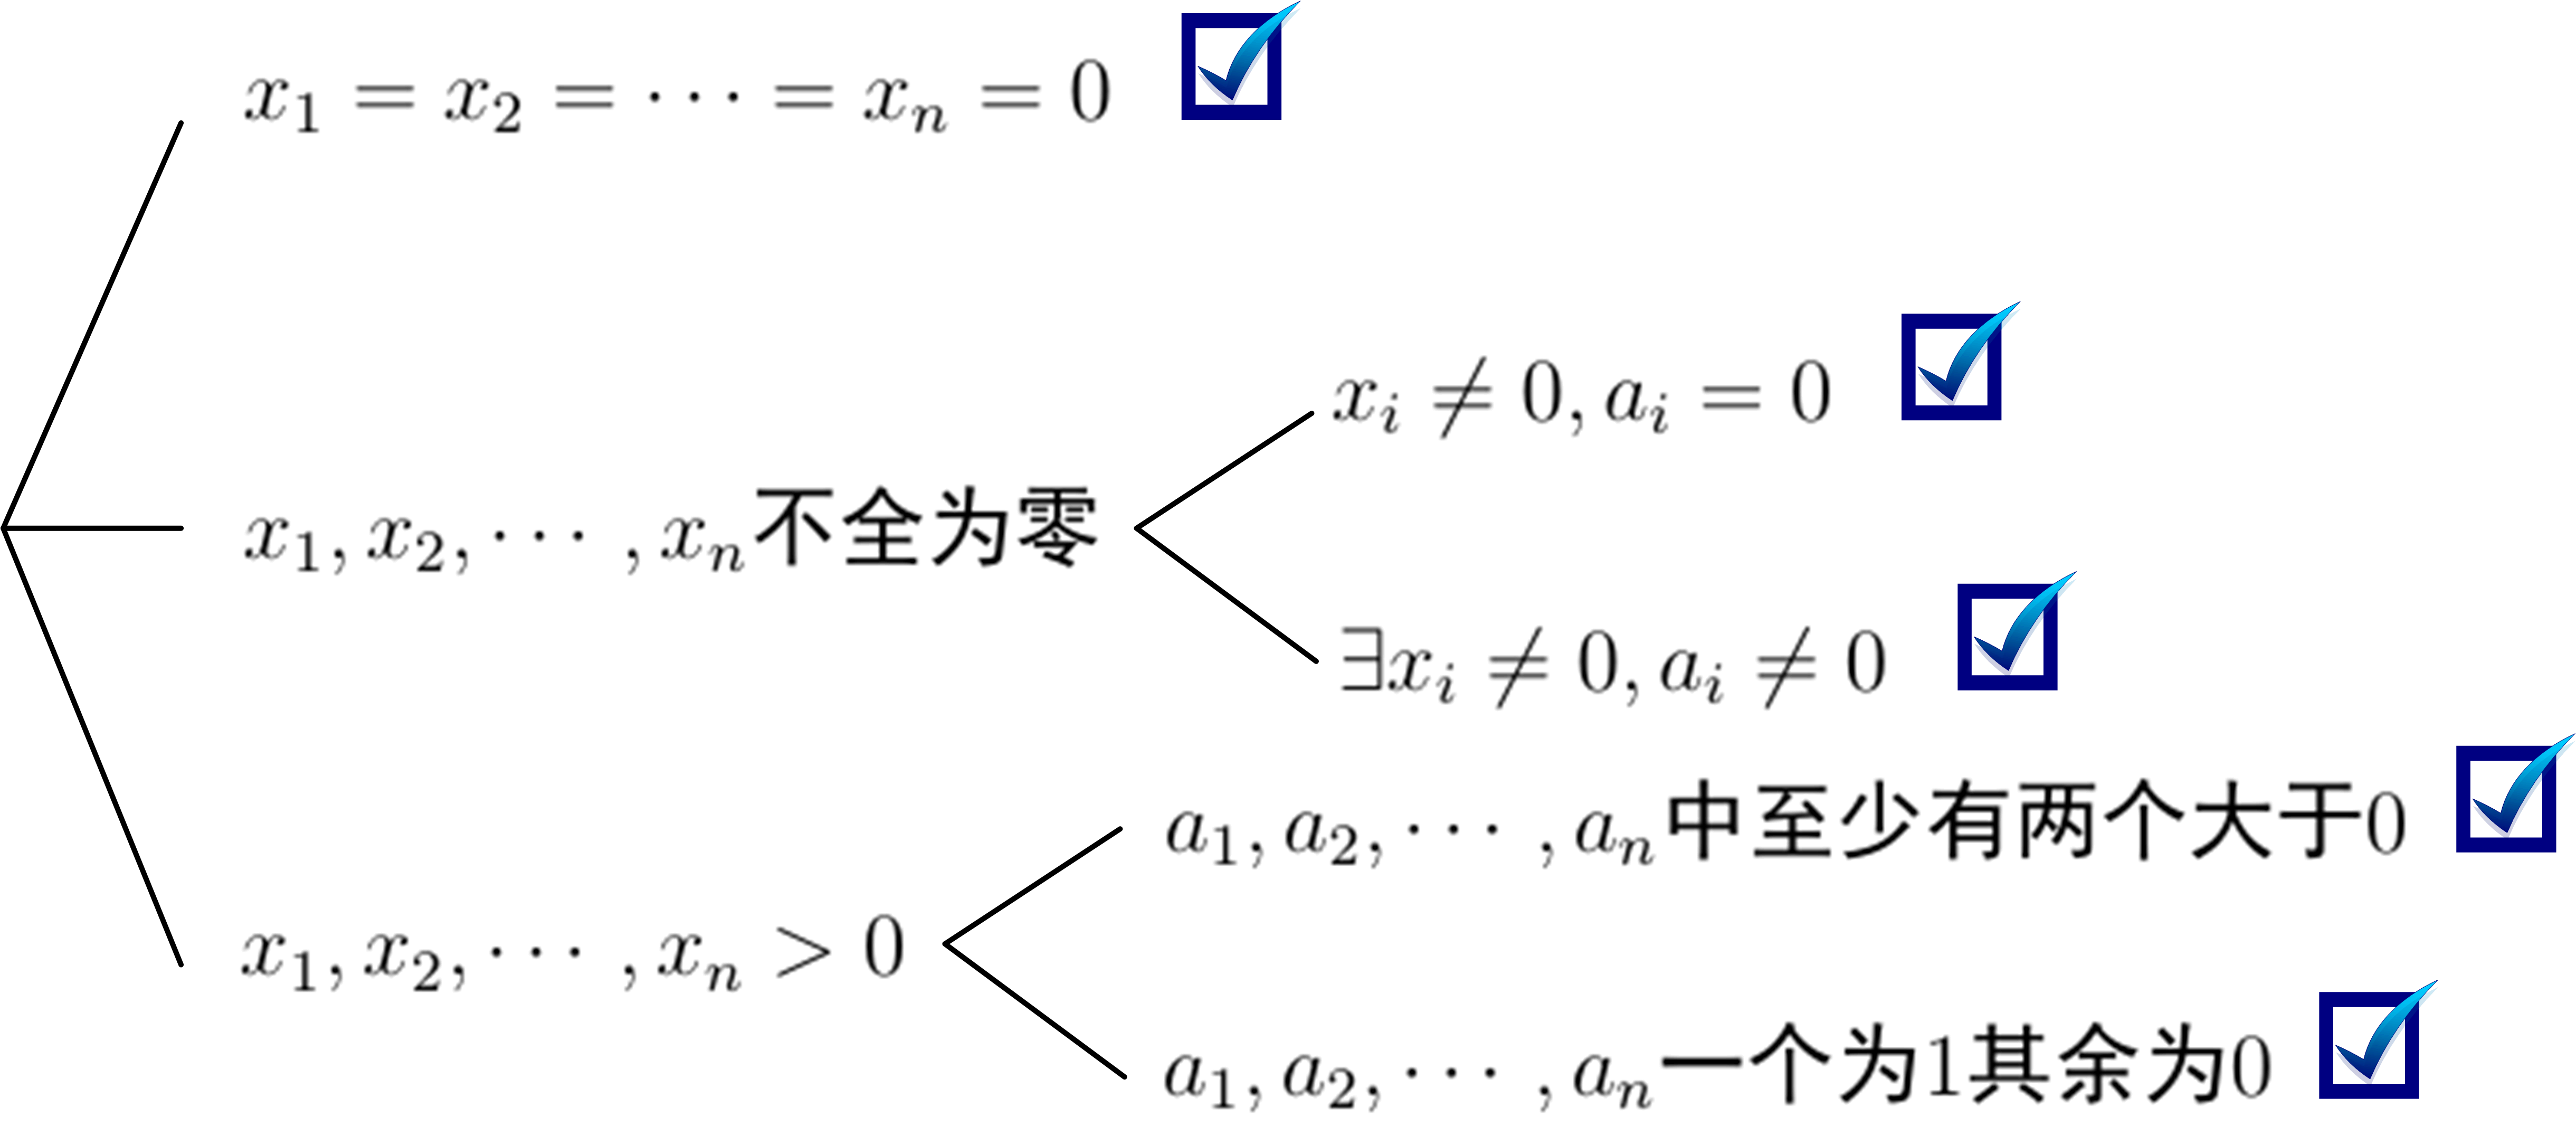
\includegraphics[height=0.2\textheight]{F:/life/2018AutumnTA/Exercises/8/Tree.png}
\end{center}
\end{figure}
对于这种问题,同时考虑$x_i,i=1,2,\cdots,n$和$a_i,i=1,2,\cdots,n$的分类不太容易. 可首先对$x_i,i=1,2,\cdots,n$进行分类,在每个$x_i$类别之下考虑$a_i,i=1,2,\cdots,n$的分类,这样会容易一些. 这也可以视为分而治之(Divide and conquer)思想的一个应用,先找到一个分类,在每一种类别之下剩余的问题可以更简单.
}

\item作下列函数的图形:
\newline
(1)$y=x^3+6x^2-15x-20$;
\newline
(2)$y=\frac{3x}{1+x^2}$;
\newline
(3)$y=\ln\frac{1+x}{1-x}$;
\newline
(4)$y=x+\arctan x$.

解:(1)i)函数的定义域为$(-\infty,+\infty)$

ii)曲线无铅直渐近线,$\lim\limits_{x\rightarrow+\infty}(x^3+6x^2-15x-20)=+\infty,\lim\limits_{x\rightarrow-\infty}(x^3+6x^2-15x-20)=-\infty$故无水平渐近线,$\lim\limits_{x\rightarrow+\infty}\frac yx=\lim\limits_{x\rightarrow+\infty}\frac{x^3+6x^2-15x-20}x=+\infty,\lim\limits_{x\rightarrow+\infty}\frac yx=\lim\limits_{x\rightarrow-\infty}\frac{x^3+6x^2-15x-20}x=-\infty$,故无斜渐近线;

iii)$y'=3x^2+12x-15=3(x^2+4x-5)=3(x+5)(x-1),y''=6x+12$,令$y'=0$得$x=-5$或$x=1$,$y''(-5)=-18<0,y''(1)=18>0$,故$(-5,80)$是函数的极大值点,$(1,-28)$是函数的极小值点,当$x=-2$时$y''=0$,故$(-2,26)$是函数的拐点

iv)当$x<-5$时$y'>0,y''<0$,函数单调增加且上凸,当$-5<x<-2$时$y'<0,y''$,当$x>1$时$y'<0,y''<0$函数单调减少且上凸,当$-2<x<1$时$y'<0,y''>0$函数单调减少且下凸,当$x>1$时$y'>0,y''>0$函数单调增加且上凸,如下表所示:
\begin{table}[H]
\centering
\begin{tabular}{c|c|c|c|c|c|c|c|c|c}
\hline
$x$ & $-\infty$ & $(-\infty,-5)$ & -5 & $(-5,-2)$ & -2 & $(-2,1)$ & 1 & $(1,+\infty)$ & $+\infty$\\
\hline
$y'$ & & + & 0 & - &  & - & 0 & + &\\
\hline
$y''$ & & - & 0 & - &  & + & 0 & + &\\
\hline
$y$ & $-\infty$ & 上凸$\nearrow$ & 极大值80 & 上凸$\searrow$ & 拐点 & 下凸$\searrow$ & 极小值-28 & 下凸$\nearrow$ & $+\infty$\\
\hline
\end{tabular}
\end{table}
可据此画出函数的略图.
\begin{figure}[H]
\begin{center}
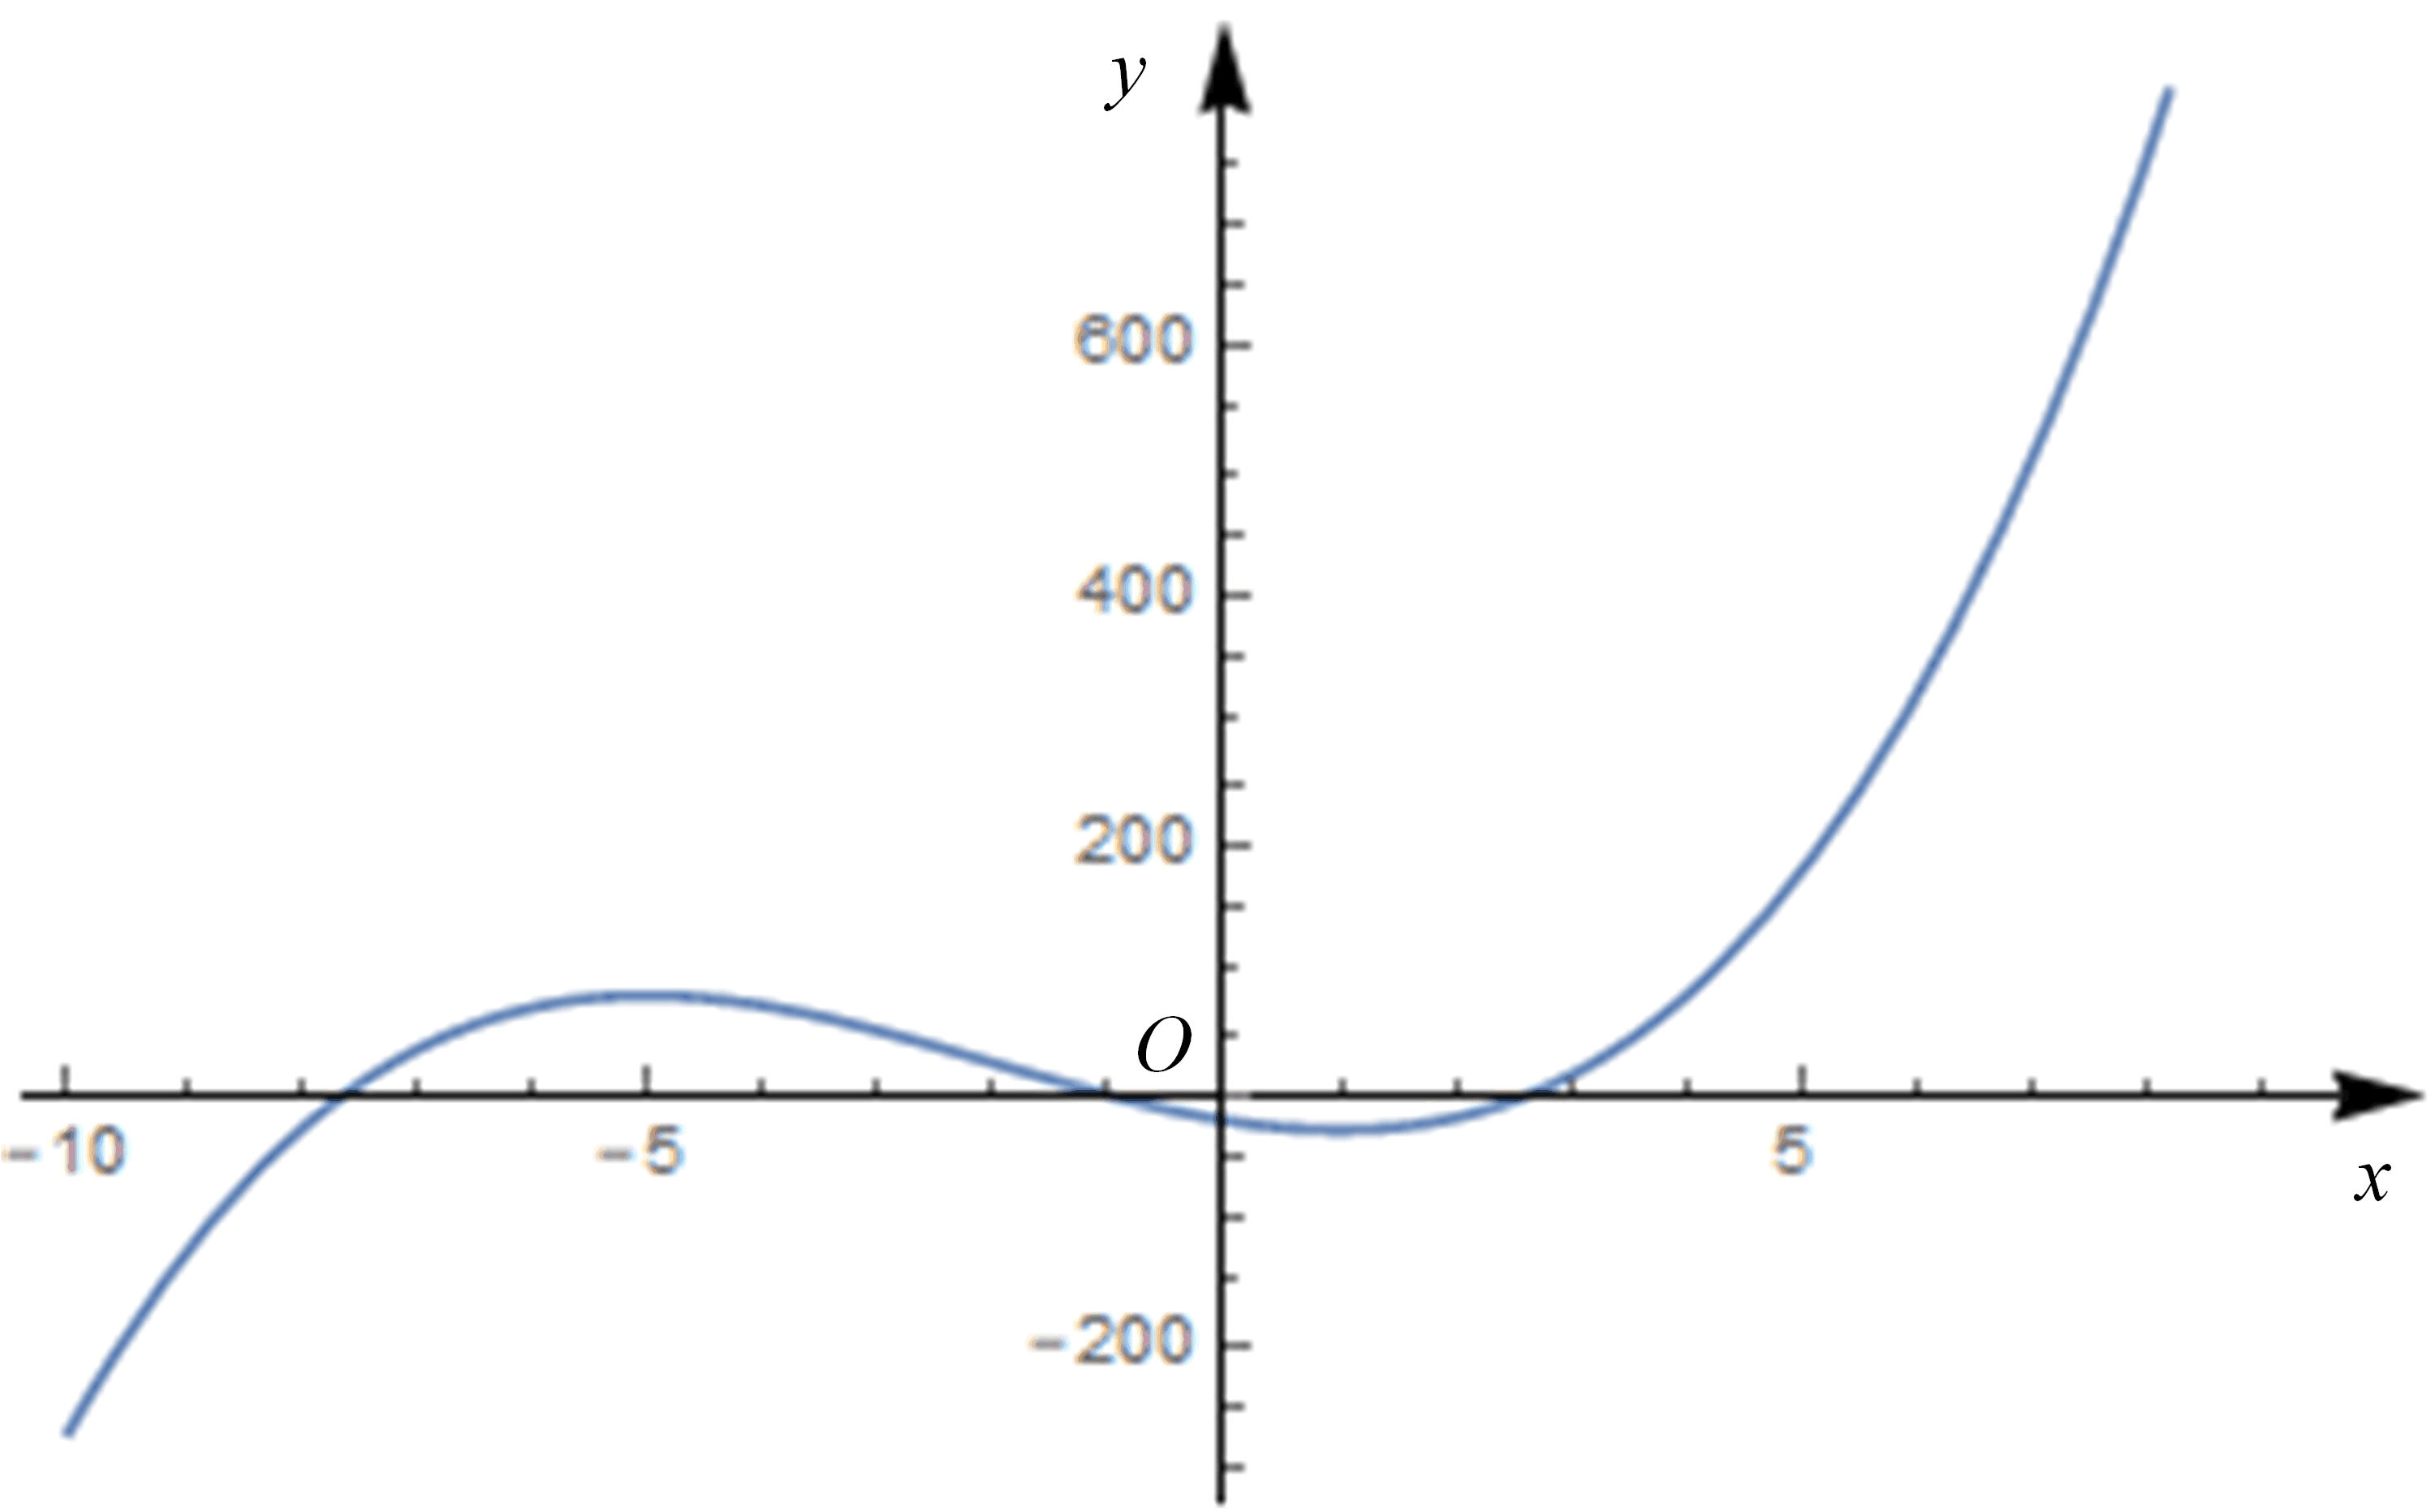
\includegraphics[height=0.2\textheight]{F:/life/2018AutumnTA/Exercises/8/Fig1-1.png}
\end{center}
\end{figure}

(2)i)函数的定义域为$(-\infty,+\infty)$,为奇函数故可仅对$[0,+\infty)$区间进行分析;

ii)$\lim\limits_{x\rightarrow\infty}\frac{3x}{1+x^2}=0$,故水平渐近线为$y=0$,$\lim\limits_{x\rightarrow\infty}\frac yx=\frac{3}{1+x^2}=0,\lim\limits_{x\rightarrow\infty}(\frac{3x}{1+x^2}-0)=0$,故无斜渐近线;

iii)$y'=\frac{3(1+x^2)-3x\cdot2x}{(1+x^2)^2}=\frac{3-3x^2}{(1+x^2)^2}=\frac{3(1-x)(1+x)}{(1+x^2)^2},y''=\frac{-6x(1+x^2)^2-[-3x^2\cdot2(1+x^2)\cdot2x]}{(1+x^2)^4}=\frac{-6x(1-x)(1+x)}{(1+x^2)^3}$. 令$y'=0$得$x=-1$或$x=1$,令$y''=0$得$x=-1$或$x=1$,函数的拐点为$(-1,-\frac32)$和$(1,\frac32)$;

iv)当$x<-1$时$y'<0,y''>0$,函数单调减少且下凸,当$-1<x<1$时$y'>0,y''<0$,函数单调增加且上凸,当$x>1$时$y'<0,y''>0$,函数单调减少且下凸. 故$(-1,-\frac32)$是函数的极小值点,$(1,\frac32)$是函数的极大值点. 如下表所示:
\begin{table}[H]
\centering
\begin{tabular}{c|c|c|c|c|c|c|c}
\hline
$x$ & $-\infty$ & $(-\infty,-1)$ & -1 & $(-1,1)$ & 1 & $(1,+\infty)$ & $+\infty$\\
\hline
$y'$ & & - & 0 & + & 0 & - &\\
\hline
$y''$ & & + & 0 & - & 0 & + & \\
\hline
$y$ & 0 & 下凸$\searrow$ & 极小值$-\frac32$、拐点 & 上凸$\nearrow$ & 极大值$\frac32$、拐点 & 下凸$\searrow$ & 1\\
\hline
\end{tabular}
\end{table}
可据此画出函数的略图.
\begin{figure}[H]
\begin{center}
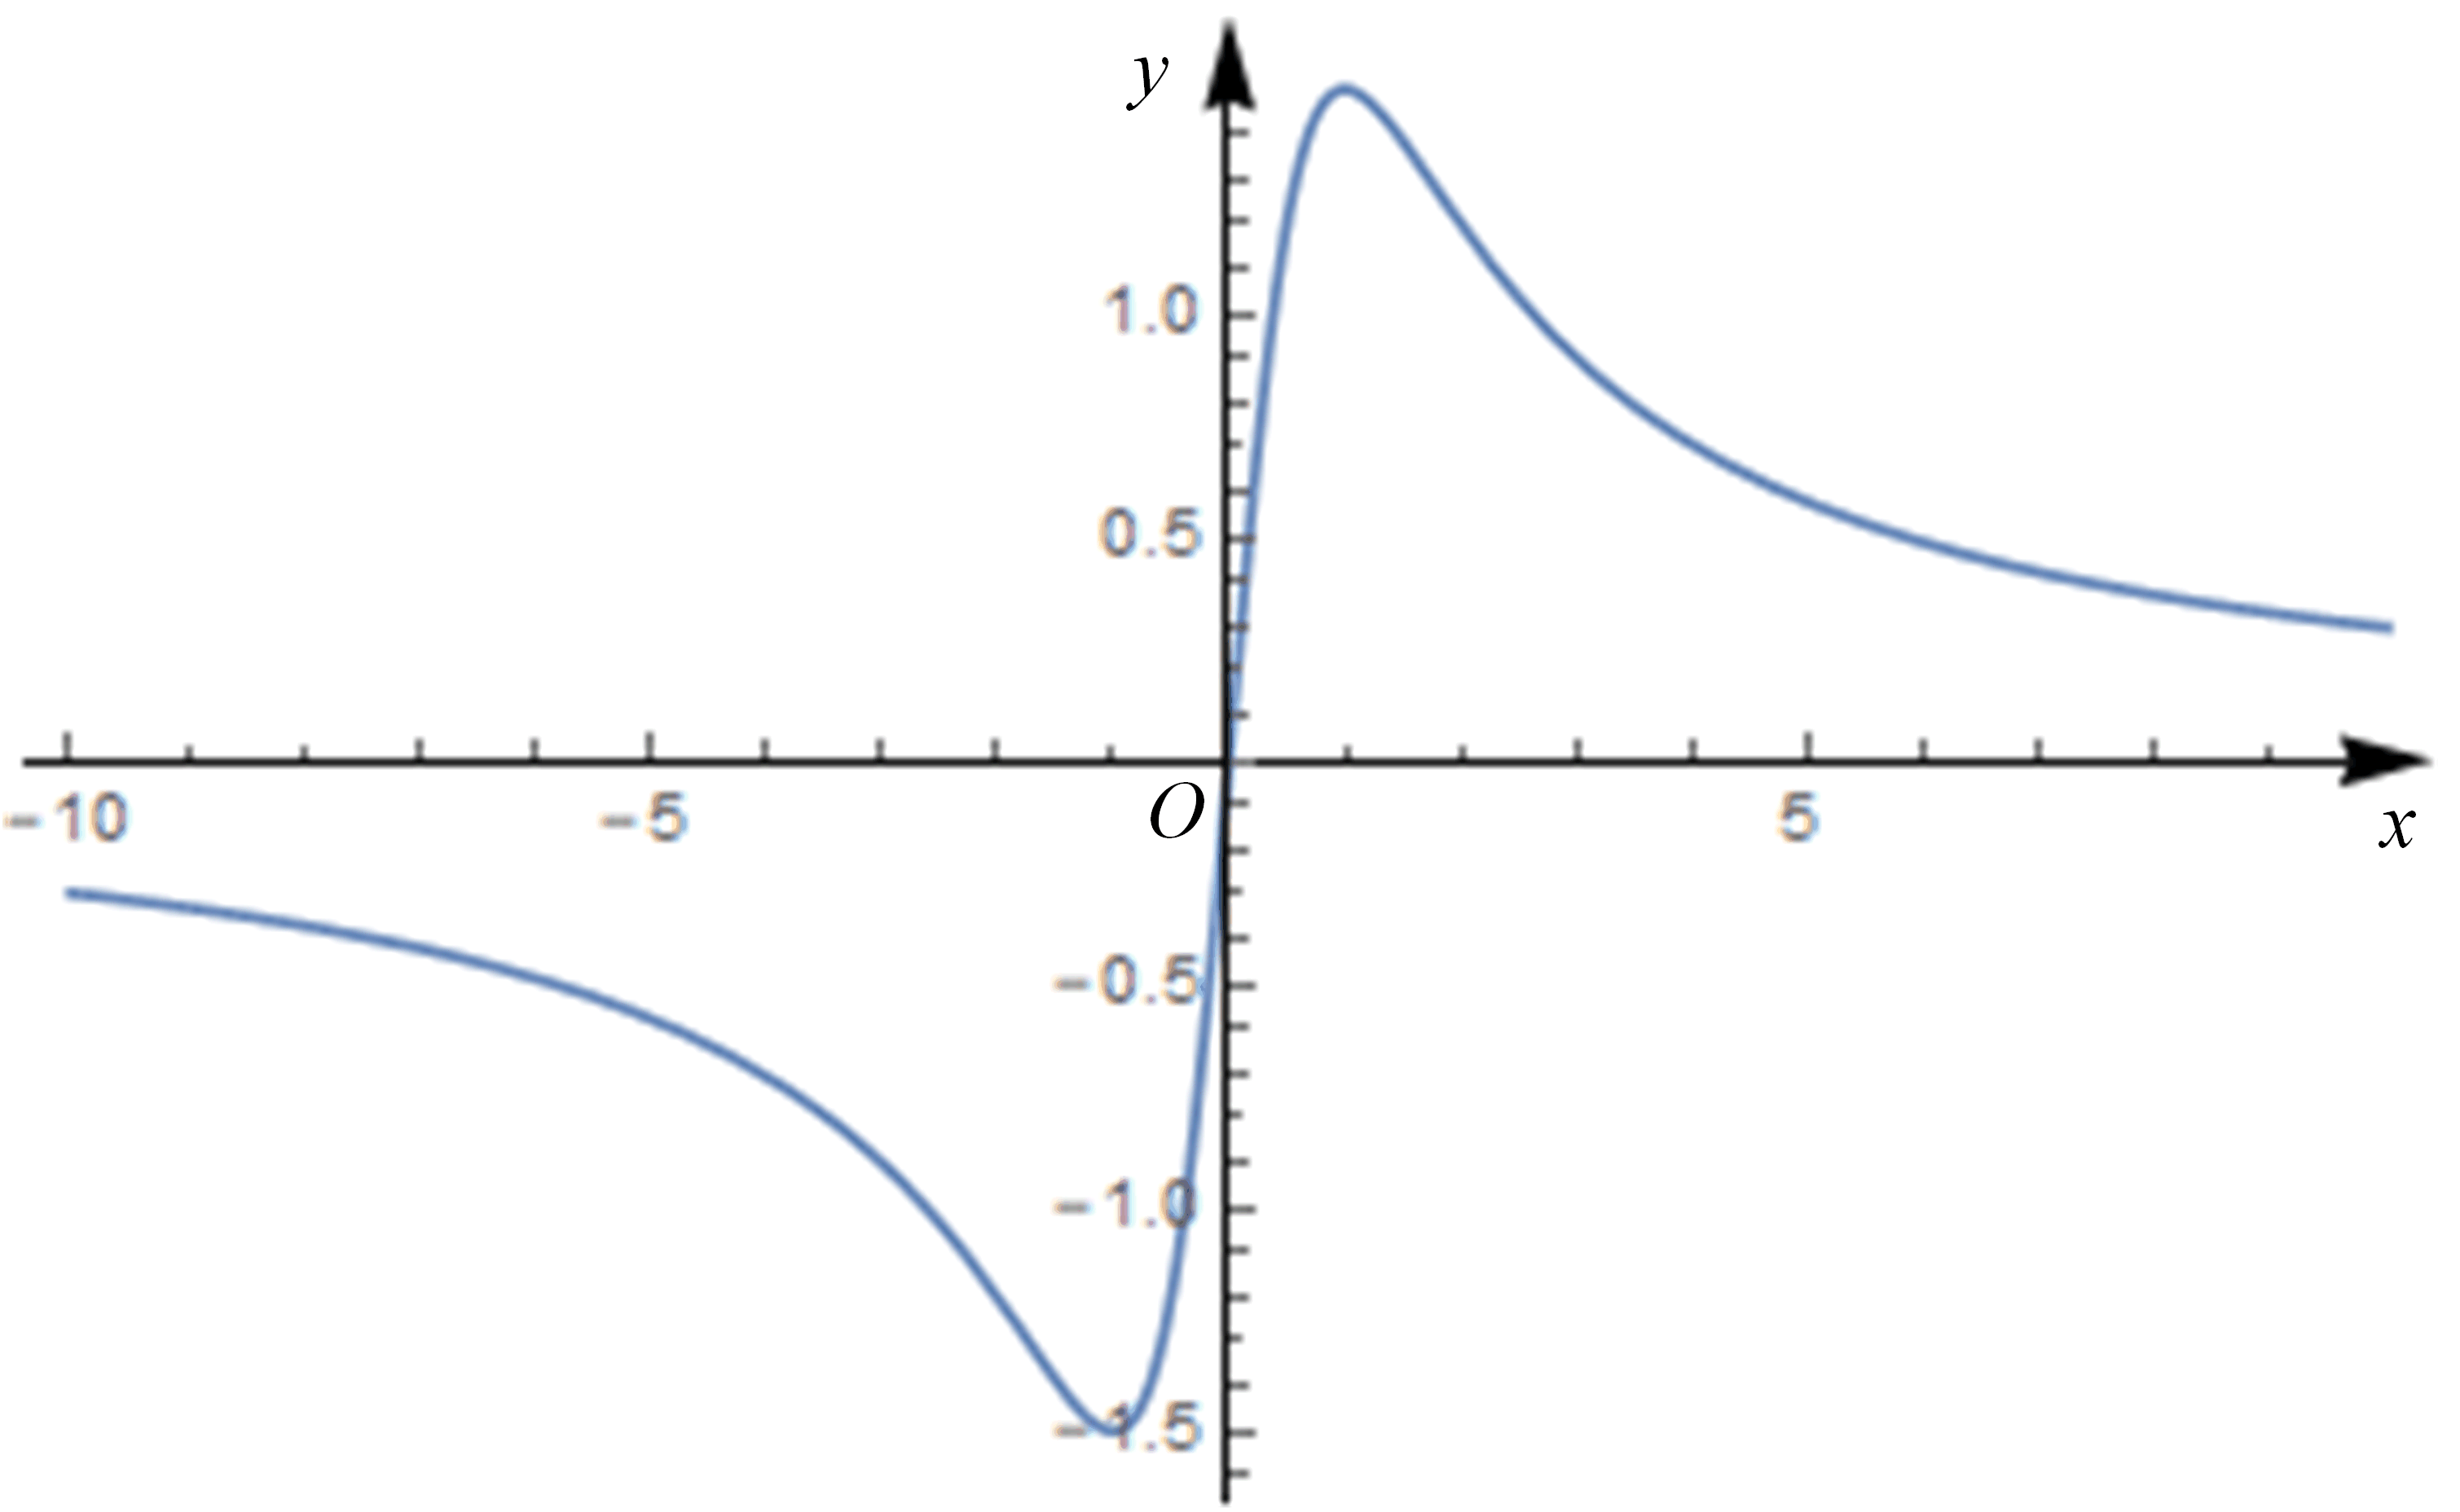
\includegraphics[height=0.2\textheight]{F:/life/2018AutumnTA/Exercises/8/Fig2-1.png}
\end{center}
\end{figure}

(3)i)由$\frac{1+x}{1-x}>0$得函数的定义域为$(-1,1)$,$y(-x)=\ln\frac{1-x}{1+x}=-\ln\frac{1+x}{1-x}=-y(x)$,故函数为奇函数;

ii)$\lim\limits_{x\rightarrow-1^+}\ln\frac{1+x}{1-x}=\lim\limits_{x\rightarrow-1^+}\ln\frac{1+x}{1-x}=-\infty,\lim\limits_{x\rightarrow1^-}\ln\frac{1+x}{1-x}=+\infty$,故函数有两条铅直渐近线$x=-1,x=1$;

iii)$y'=\frac1{1+x}+\frac1{1-x}=\frac2{(1-x)(1+x)}>0,y''=\frac{-1}{(1+x)^2}+\frac1{(1-x)^2}=\frac{4x}{(1-x)^2(1+x)^2}$,当$x=0$时$y''=0$,故函数的拐点为$(0,0)$;

iv)当$-1<x<0$时$y''<0$,函数单调增加且上凸,当$0<x<1$时,函数单调减少且下凸. 如下表所示:
\begin{table}[H]
\centering
\begin{tabular}{c|c|c|c|c|c}
\hline
$x$ & -1 & $(-1,0)$ & 0 & $(0,1)$ & 1 \\
\hline
$y'$ &  & + & 2 & + & \\
\hline
$y''$ &  & - & 0 & + & \\
\hline
$y$ & $-\infty$ & 上凸$\nearrow$ & 拐点 & 下凸$\nearrow$ & +$\infty$\\
\hline
\end{tabular}
\end{table}
可据此画出函数的略图.
\begin{figure}[H]
\begin{center}
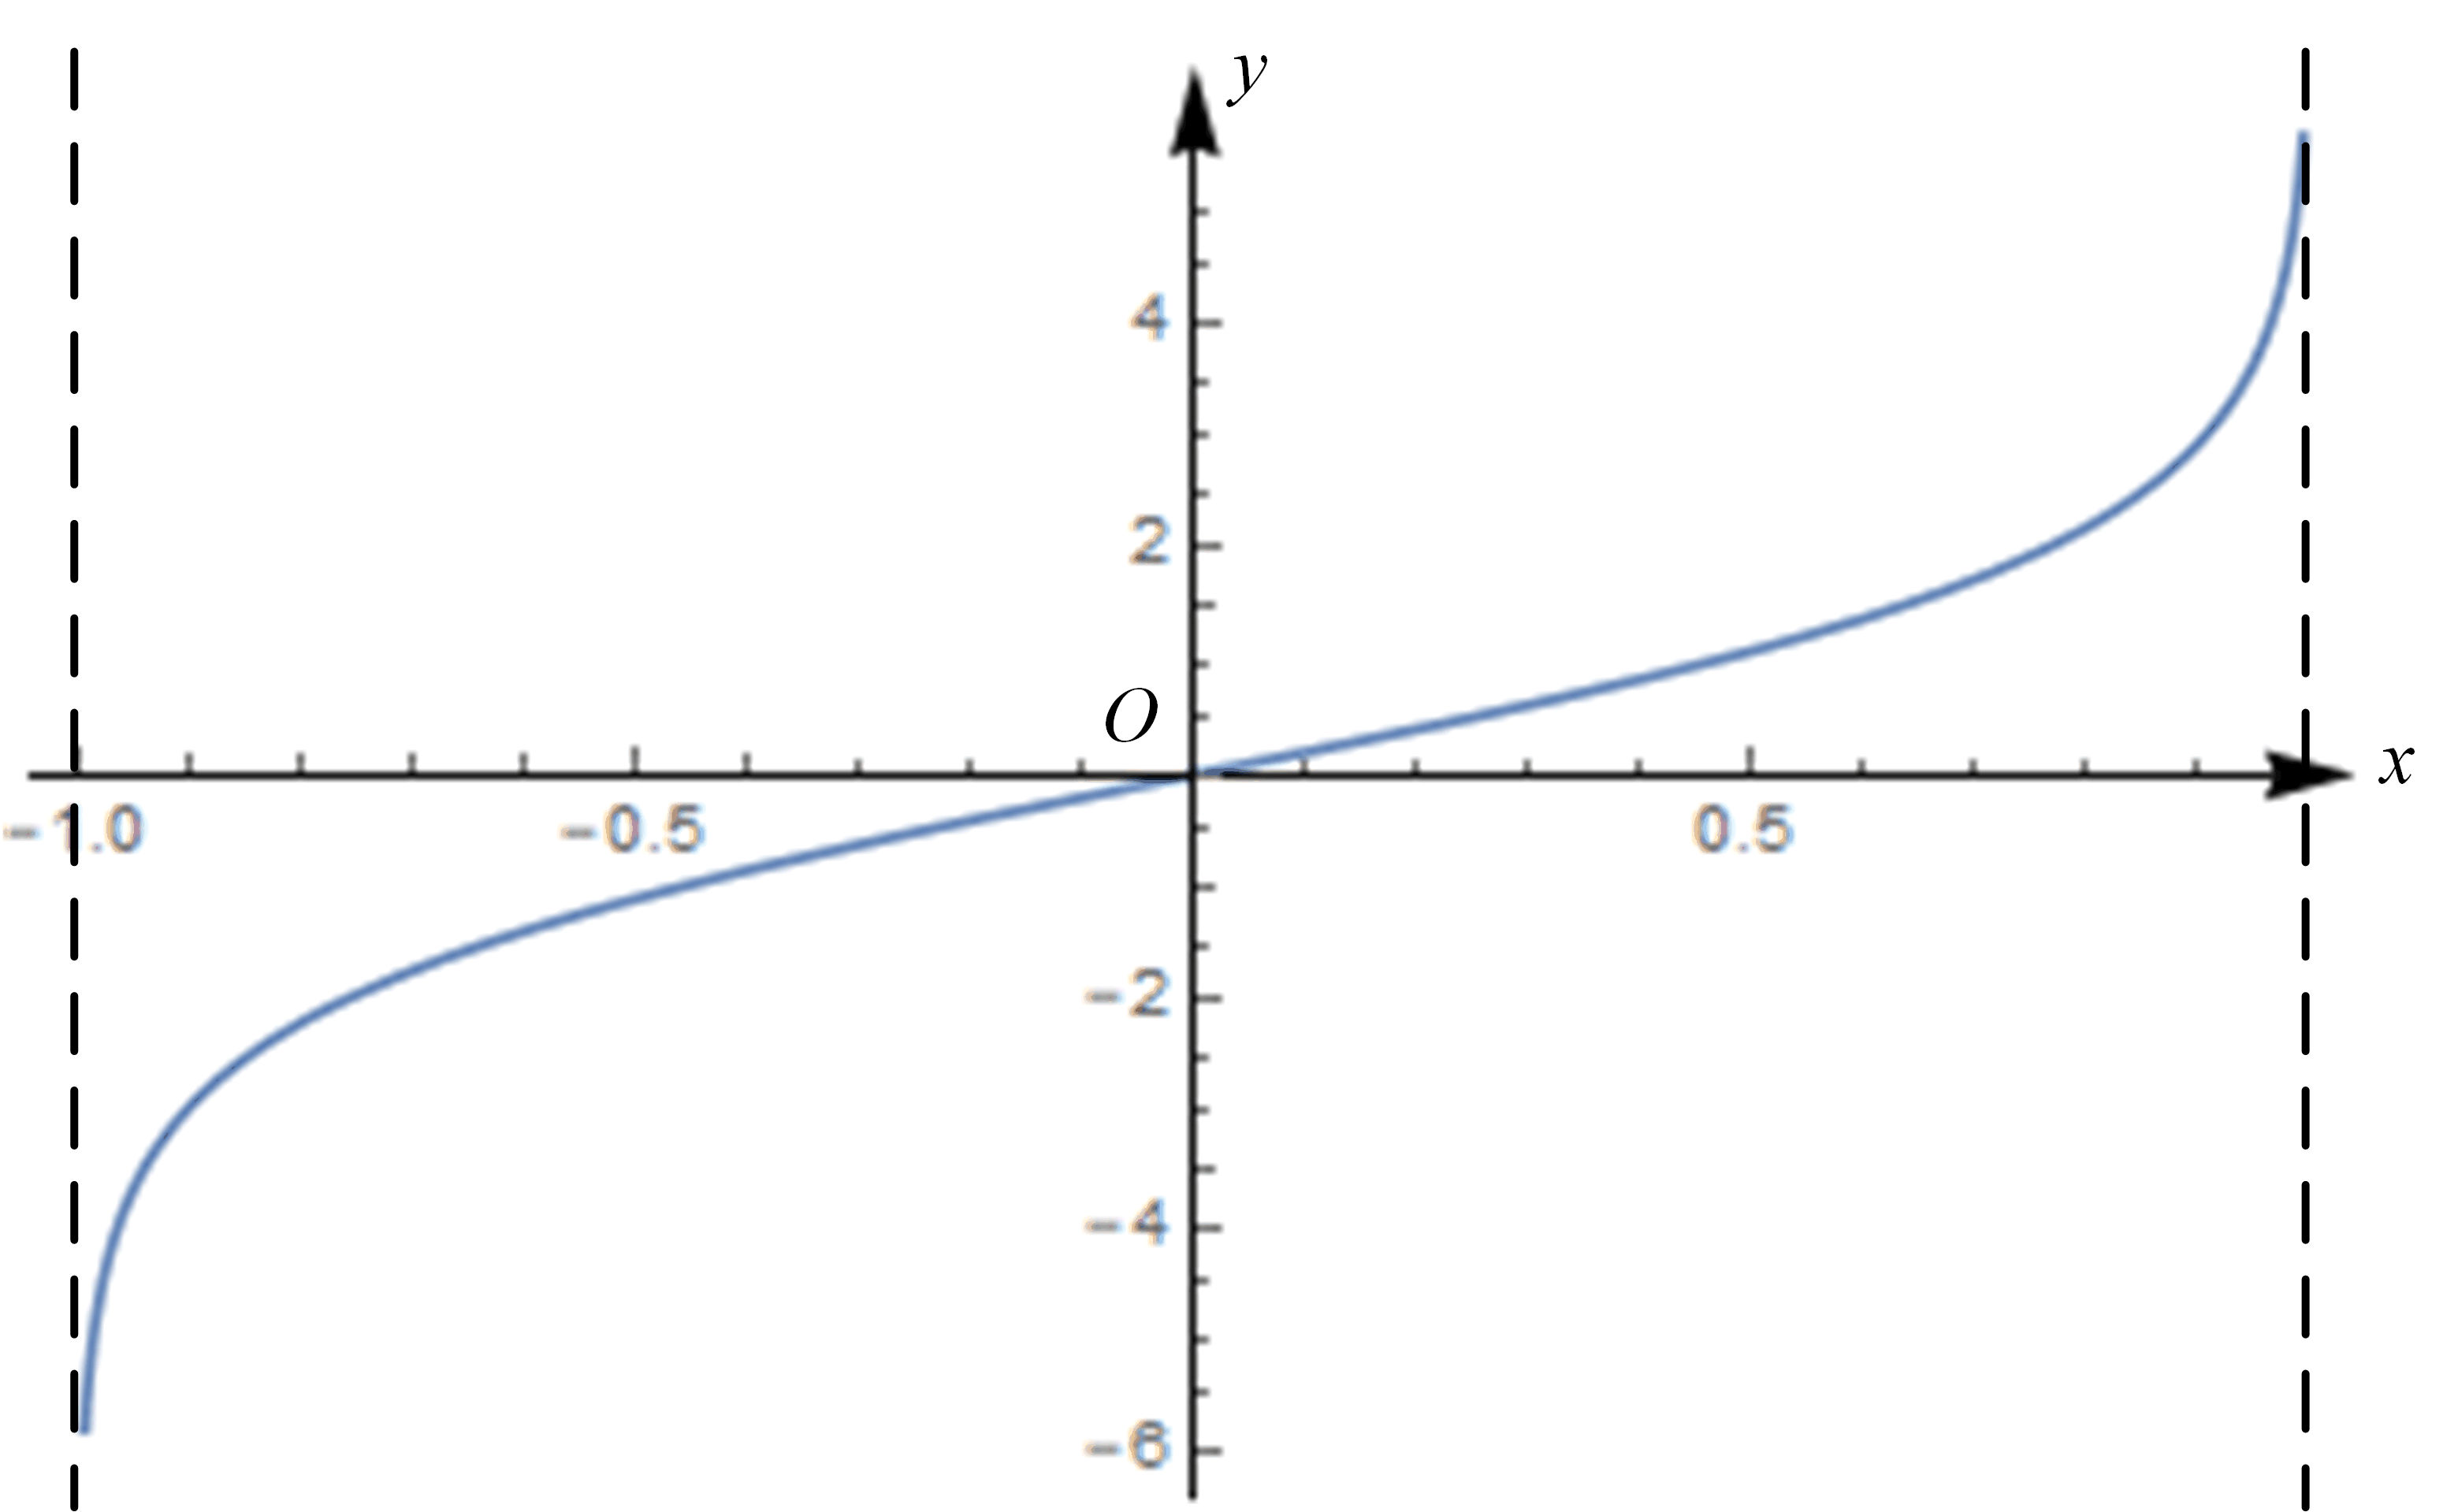
\includegraphics[height=0.2\textheight]{F:/life/2018AutumnTA/Exercises/8/Fig3-1.png}
\end{center}
\end{figure}

(4)i)函数的定义域为$(-\infty,+\infty)$,易知函数为奇函数;

ii)函数无铅直渐近线,$\lim\limits_{x\rightarrow+\infty}(x+\arctan x)=+\infty,\lim\limits_{x\rightarrow-\infty}(x+\arctan x)=-\infty$,故无水平渐近线,$\lim\limits_{x\rightarrow+\infty}\frac yx=\lim\limits_{x\rightarrow+\infty}\frac{x+\arctan x}x=1,\lim\limits_{x\rightarrow+\infty}(y-x)=\lim\limits_{x\rightarrow+\infty}\arctan x=\frac\pi2$,故有斜渐近线$y=x+\frac\pi2$和$y=x-\frac\pi2$;

iii)$y'=1+\frac1{1+x^2}>0,y''=-\frac{2x}{(1+x^2)^2}$,函数有一个拐点$(0,0)$;

iv)当$x<0$时$y''>0$函数单调增加且下凸,当$x>0$时$y''<0$,函数单调增加且下凸. 如下表所示:
\begin{table}[H]
\centering
\begin{tabular}{c|c|c|c|c|c}
\hline
$x$ & $-\infty$ & $(-\infty,0)$ & 0 & $(0,+\infty)$ & $+\infty$\\
\hline
$y'$ & & + &  & + &\\
\hline
$y''$ & & - & 0 & + &\\
\hline
$y$ & $x-\frac\pi2$ & 上凸$\nearrow$ & 拐点 & 下凸$\nearrow$ & $x+\frac\pi2$\\
\hline
\end{tabular}
\end{table}

可据此画出函数的略图.
\begin{figure}[H]
\begin{center}
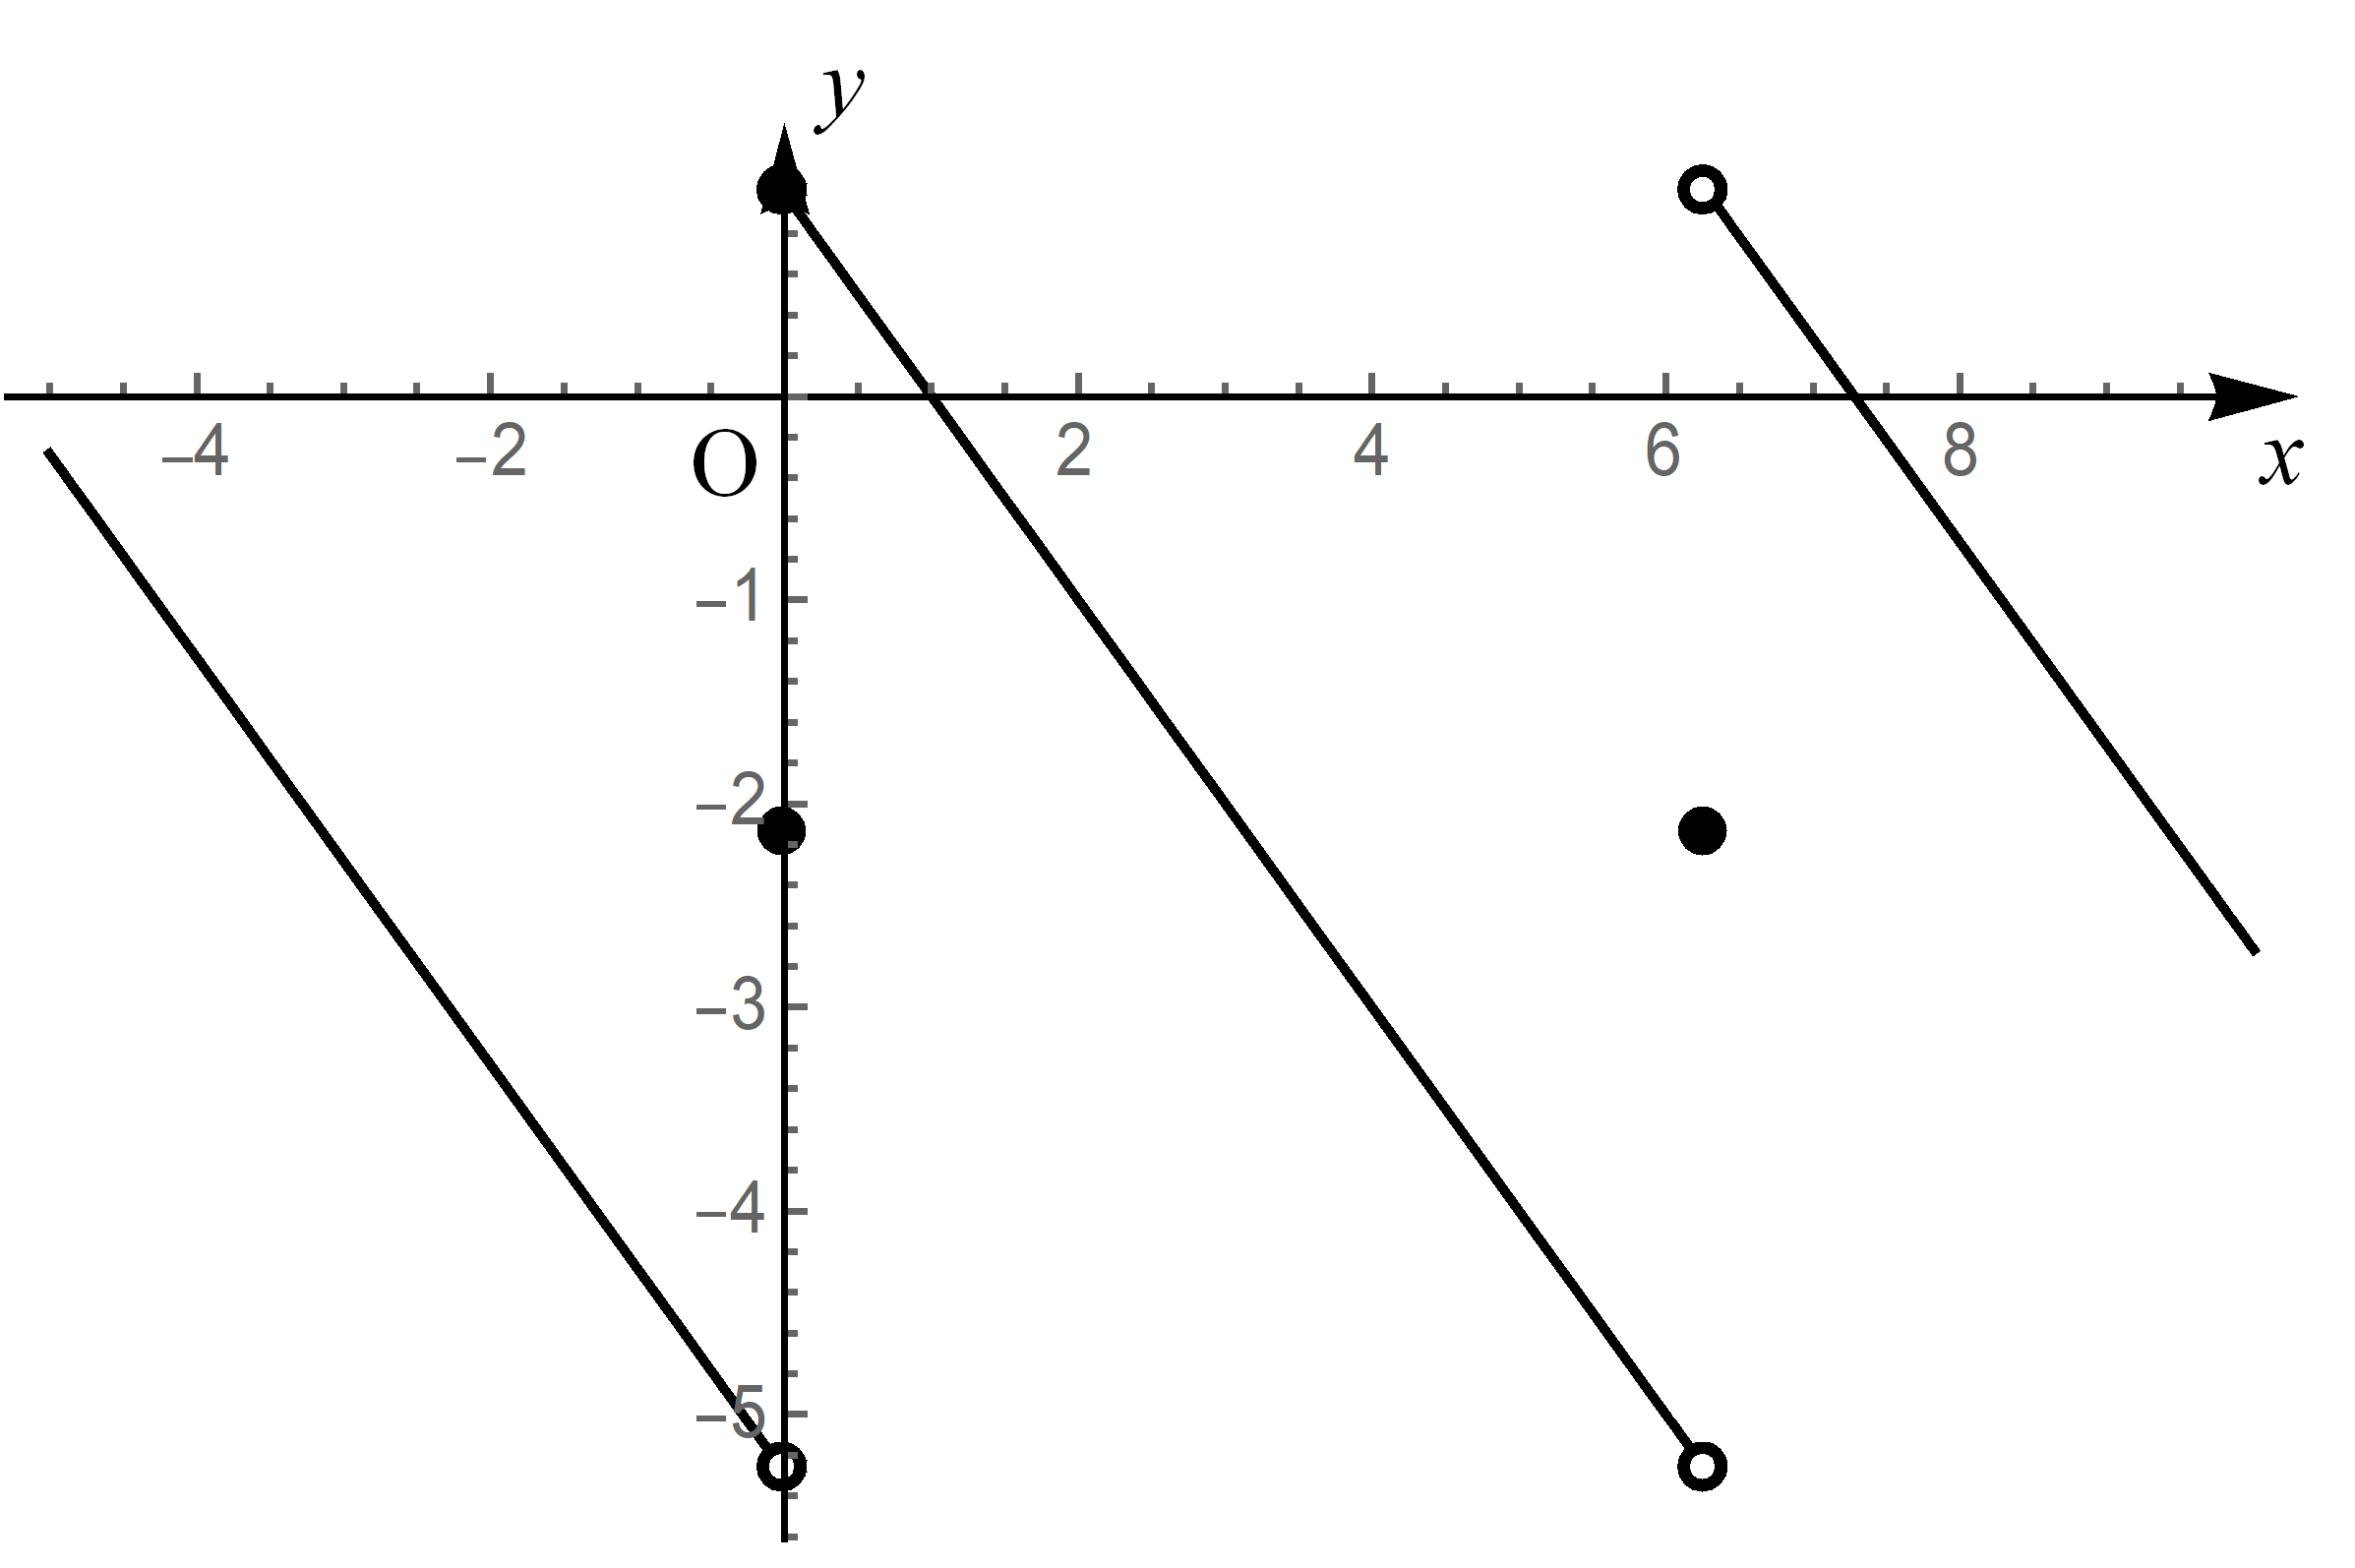
\includegraphics[height=0.2\textheight]{F:/life/2018AutumnTA/Exercises/8/Fig4-1.png}
\end{center}
\end{figure}

\item已知$y=f(x)$是由方程$y^3-x^3+2xy=0$所确定的隐函数,设曲线$y=y(x)$有斜渐近线$y=ax+b$,求$a,b$.

解:$\because$曲线有斜渐近线

$\therefore\lim\limits_{x\rightarrow+\infty}\frac yx=a$存在

将方程$y^3-x^3+2xy=0$两边同除以$x^3$并取极限得$a^3-1-0=0$,故$a=1$

将$y^3-x^3+2xy=(x-y)(x^2+xy+y^2)+2xy=0$两边同除以$x^2$并取极限得$[\lim\limits_{x\rightarrow+\infty}(x-y)](1+a+a^2)+2a=0$,故$b=-\lim\limits_{x\rightarrow+\infty}(x-y)=\frac{-2a}{1+a+a^2}=-\frac23$.
\end{enumerate}
\subsection{习题5.5解答}
\begin{enumerate}
\item按指定次数写出下列函数在指定点的泰勒多项式:
\newline
(1)$f(x)=\frac{1+x+x^2}{1-x+x^2},x_0=0$,展到4次;
\newline
(2)$f(x)=\ln\cos x,x_0=0$,展到6次;
\newline
(3)$f(x)=\sqrt x,x_0=1$,展到4次;
\newline
(4)$f(x)=1+2x-4x^2+x^3+6x^4,x_0=1$,展到6次;
\newline
(5)$f(x)=\frac x{x-1},x_0=2$,展到$n$次;
\newline
(6)$f(x)=x^3\ln x,x_0=1$,展到5次.

解:(1)方法1:$f(x)(1-x+x^2)=1+x+x^2,f(0)=1$

$f'(x)(1-x+x^2)+f(x)(-1+2x)=1+2x,f'(0)=2$

$f''(x)(1-x+x^2)+2f'(x)(-1+2x)+f(x)2=2,f''(0)=4$

$f'''(x)(1-x+x^2)+3f''(x)(-1+2x)+3f'(x)2=0,f'''(0)=0$

$f^{(4)}(x)(1-x+x^2)+4f'''(x)(-1+2x)+6f''(x)2=0,f''''(0)=-48$

$\therefore f(x)=f(0)+f'(0)x+\frac{f''(0)}{2!}x^2+\frac{f'''(0)}{3!}x^3+\frac{f''''(0)}{4!}x^4+o(x^4)=1+2x+2x^2-2x^4+o(x^4)$.

方法2:
\[\begin{split}
f(x)&=\frac{1+x+x^2}{1-x+x^2}=\frac{(1+x+x^2)(x-1)}{(1-x+x^2)(x+1)}\frac{x+1}{x-1}\\
&=\frac{x^3-1}{x^3+1}\frac{x+1}{x-1}=(1-\frac2{1+x^3})(1-\frac2{1-x})\\
&=\{1-2[\sum_{k=0}^n(-x^3)^k+o(x^{3n})]\}\{1-2[\sum_{k=0}^nx^k+o(x^n)]\}\\
&=\{1-2[1-x^3+o(x^4)]\}\{1-2[1+x+x^2+x^3+x^4+o(x^4)]\}\\
&=[-1+2x^3+o(x^4)][-1-2x-2x^2-2x^3-2x^4+o(x^4)]\\
&=1+2x+2x^2+(2-2)x^3+(2-4)x^4+o(x^4)\\
&=1+2x+2x^2-2x^4+o(x^4).
\end{split}\]
(2)方法1:$f(x)=\ln\cos x,f(0)=0$

$f'(x)=\frac{-\sin x}{\cos x}=-\tan x,f'(0)=0$

$f''(x)=-\sec^2x,f''(0)=-1$

$f'''(x)=-2\sec x\sec x\tan x=2\sec^2x\tan x,f'(0)=0$

$f^{(4)}(x)=-4\sec x\sec x\tan x\tan x-2\sec^2x\sec^2x=-2\sec^2x(2\tan^2x+\sec^2x),f''''(0)=-2$

$f^{(5)}(x)=-4\sec x\sec x\tan x(2\tan^2x+\sec^2x)-2\sec^2x(4\tan x\sec^2x+2\sec x\sec x\tan x)=-4\sec^2x\tan x(2\tan^2x+\sec^2x)-2\sec^2x(6\tan x\sec^2x)=-8\sec^2x\tan^3x-16\sec^4x\tan x=-8\sec^2x\tan x(\tan^2x+2\sec^2x),f^{(5)}(0)=0$

$f^{(6)}=-(16\sec x\tan x+8\sec^4x)(\tan^2x+2\sec^2x)-8\sec^2x\tan x(2\tan x\sec^2x+4\sec x\sec x\tan x),f^{(6)}(0)=-16$

$\therefore f(x)=-\frac12x^2-\frac1{12}x^4-\frac1{45}x^6+o(x^6)$.

方法2:\[\begin{split}
f(x)&=\ln\cos x=\ln[1+(\cos x-1)]\\
&=\sum_{k=1}^n\frac{(-1)^{k-1}}k(\cos x-1)^k+o((\cos x-1)^n)\\
&=\sum_{k=1}^n\frac{(-1)^{k-1}}k[\sum_{i=0}^m\frac{(-1)^{2i}}{(2i)!}x^{2i}+o(x^{2m+1})-1]^k+o(x^{2mn})\\
&=\sum_{k=1}^3\frac{(-1)^{k-1}}k[-\frac1{2!}x^2+\frac1{4!}x^4-\frac1{6!}x^6+o(x^6)]^k+o(x^{18})\\
&=-\frac1{2!}x^2+\frac1{4!}x^4-\frac1{6!}x^6+o(x^6)-\frac12[\frac14x^4-2\cdot\frac1{2!\cdot4!}x^6+o(x^6)]+\frac13[-\frac18x^6+o(x^6)]+o(x^{18})\\
&=-\frac12x^2+(\frac1{24}-\frac18)x^4+(-\frac1{720}+\frac1{48}-\frac1{24})x^6+o(x^6)\\
&=-\frac12x^2-\frac1{12}x^4-\frac1{45}x^6+o(x^6).
\end{split}\]
(3)方法1:$f(x)=\sqrt x,f(1)=1$

$f'(x)=\frac1{2\sqrt x},f'(1)=\frac12$

$f''(x)=\frac{-1}{4x^{\frac32}},f''(1)=-\frac14$

$f'''(x)=\frac{3}{8x^{\frac52}},f'''(1)=\frac38$

$f^{(4)}=\frac{-15}{16x^{\frac72}},f^{(4)}=-\frac{15}{16}$

$\therefore f(x)=f(1)+f'(1)(x-1)+\frac{f''(1)}{2!}(x-1)^2+\frac{f'''(1)}{3!}(x-1)^3+\frac{f^{(4)}(1)}{4!}(x-1)^4+o(x^4)=1+\frac12(x-1)-\frac18(x-1)^2+\frac1{16}-\frac5{128}(x-1)^4+o((x-1)^4)$.

方法2:\[\begin{split}
f(x)&=\sqrt x=\sqrt{1+(x-1)}\\
&=1+\sum_{k=1}^n\frac{\frac12(-\frac12)(-\frac32)\cdots(\frac12-k+1)}{k!}(x-1)^k+o((x-1)^n)\\
&=1+\frac12(x-1)+\frac{\frac12(-\frac12)}2(x-1)^2+\frac{\frac12(-\frac12)(-\frac32)}6(x-1)^3+\frac{\frac12(-\frac12)(-\frac32)(-\frac52)}{24}(x-1)^4\\
&\hspace{1cm}+o((x-1)^4)\\
&=1+\frac12(x-1)-\frac18(x-1)^2+\frac1{16}(x-1)^3-\frac5{128}(x-1)^4+o((x-1)^4)
\end{split}\]
(4)$f(x)=1+2x-4x^2+x^3+6x^4,f(1)=1+2-4+1+6=6$

$f'(x)=2-8x+3x^2+24x^3,f'(1)=2-8+3+24=21$

$f''(x)=-8+6x+72x^2,f''(1)=-8+6+72=70$

$f'''(x)=6+144x,f'''(1)=150$

$f^{(4)}(x)=144$

$f^{(5)}(x)=0$

$f^{(6)}(x)=0$

$f(x)=6+21(x-1)+35(x-1)^2+25(x-1)^3+6(x-1)^4+o((x-1)^6)$.

(5)$f(x)=\frac x{x-1},f(2)=2$

$f'(x)=\frac{(x-1)-x}{(x-1)^2}=\frac{-1}{(x-1)^2},f'(2)=-1$

$f''(x)=\frac{2}{(x-1)^3},f''(2)=2$

$f^{(n)}(x)=\frac{(-1)^nn!}{(x-1)^{n+1}}$

$f(x)=f(2)+\sum_{k=1}^n\frac{f^{(k)}}{k!}(x-1)^{k}=2+\sum_{k=1}^n\frac{(-1)^kk!}{k!}(x-1)^{k}=2+\sum_{k=1}^n(-1)^k(x-1)^{k}$.

方法2:\[\begin{split}
f(x)&=\frac x{x-1}=\frac{x-1+1}{x-1}=1+\frac1{x-1}=1+\frac1{1+(x-2)}\\
&=1+\sum_{k=0}^n[-(x-2)]^k+o((x-2)^n)\\
&=2+\sum_{k=1}^n[-(x-2)]^k+o((x-2)^n)
\end{split}\]
(6)方法1:$f(x)=x^3\ln x,f(1)=0$

$f'(x)=3x^2\ln x+x^3\frac1x=x^2(3\ln x+1),f'(1)=1$

$f''(x)=2x(3\ln x+1)+x^2\frac3x=x(6\ln x+5),f''(1)=5$

$f'''(x)=6\ln x+5+x\frac6x=6\ln x+11,f'''(1)=11$

$f^{(4)}(x)=\frac6x,f^{(4)}(1)=6$

$f^{(5)}(x)=-\frac6{x^2},f^{(5)}(1)=-6$

$f(x)=f(1)+f'(1)(x-1)+\frac{f''(1)}{2!}(x-1)^2+\frac{f'''(1)}{3!}(x-1)^3+\frac{f^{(4)}(1)}{4!}(x-1)^4+\frac{f^{(5)}(1)}{5!}(x-1)^5+o((x-1)^5)=(x-1)+\frac52(x-1)^2+\frac{11}6(x-1)^3+\frac14(x-1)^4-\frac1{20}(x-1)^5+o((x-1)^5)$.

方法2:\[\begin{split}
f(x)&=x^3\ln x=[1+(x-1)]^3\ln[1+(x-1)]\\
&=[1+3(x-1)+\frac{3\cdot2}{2!}(x-1)^2+\frac{3\cdot2\cdot1}{3!}(x-1)^3][\sum_{k=1}^n\frac{(-1)^{k-1}}k(x-1)^k+o((x-1)^n)]\\
&=[1+3(x-1)+3(x-1)^2+(x-1)^3][(x-1)-\frac12(x-1)^2+\frac13(x-1)^3-\frac14(x-1)^4\\
&\hspace{1cm}+\frac15(x-1)^5+o((x-1)^5)]\\
&=(x-1)+(3-\frac12)(x-1)^2+(\frac13-\frac32+3)(x-1)^3+(1-\frac32+1-\frac14)(x-1)^4\\
&\hspace{1cm}+(-\frac12+1-\frac34+\frac15)(x-1)^5+o((x-1)^5)\\
&=(x-1)+\frac52(x-1)^2+\frac{11}6(x-1)^3+\frac14(x-1)^4-\frac1{20}(x-1)^5+o((x-1)^5).
\end{split}\]
\item设函数$f(x)$在点$x_0$附近有$n+1$阶连续导数且$f'(x_0)=\cdots=f^{(n)}(x_0)=0,f^{(n+1)}(x_0)\neq0$,证明:若$n$为奇数,则点$x_0$是$f(x)$的极值点;若$n$为偶数,则点$x_0$不是$f(x)$的极值点.

证明:{\bf方法1:}$\because f(x)$在点$x_0$附近有$n+1$阶连续导数且$f'(x_0)=\cdots=f^{(n)}(x_0)=0,f^{(n+1)}(x_0)\neq0$

$\therefore$在$x_0$的某个去心邻域$N^*(x_0)$内$f^{(n+1)}(x)\neq0$且在该邻域内$f(x)=f(x_0)+\frac{f^{(n+1)}(\xi)}{(n+1)!}(x-x_0)^{n+1}$,$\xi$介于$x$和$x_0$之间

{\bf正确做法:}当$n$为奇数时,在$N^*(x_0)$内$f(x)-f(x_0)=\frac{f^{(n+1)}(\xi)}{(n+1)!}(x-x_0)^{n+1}$与$f^{(n+1)}(\xi)$同号,故$x_0$是$f(x)$的极值点;当$n$为偶数时,在$N^*(x_0)$内$f(x)-f(x_0)=\frac{f^{(n+1)}(\xi)}{(n+1)!}(x-x_0)^{n+1}$在$x_0$两侧异号,故$x_0$不是$f(x)$的极值点. 

{\bf可能有问题的做法:}{\bf\color{red}{$\therefore f'(x)=\frac{f^{(n+1)}(\xi)}{n!}(x-x_0)^n$}

当$n$为偶数时$f'(x)$在$x_0$两侧附近同号,故点$x_0$不是$f(x)$的极值点;当$n$为奇数时$f'(x)$在$x_0$两侧附近异号,故点$x_0$是$f(x)$的极值点.}

{\bf\color{red}这样做可能有问题,因为$f^{(n+1)}(\xi)$与$x$有关,求导后不一定等于0,即$f'(x)=\frac{f^{(n+1)}(\xi)}{n!}(x-x_0)^n+(\frac{f^{(n+1)}(\xi)}{(n+1)!})'(x-x_0)^{n+1}$}

{\bf方法2:}由$f(x)=\sum_{k=0}^n\frac{f^{(k)}(x_0)}{k!}(x-x_0)^k+o((x-x_0)^n)$及$f'(x_0)=\cdots=f^{(n)}(x_0)=0,f^{(n+1)}(x_0)\neq0$可知
\[
f(x)-f(x_0)=\frac{f^{(n+1)}(x_0)}{(n+1)!}(x-x_0)^{n+1}+o((x-x_0)^{n+1}),
\]
则\[
\lim\limits_{x\rightarrow x_0}\frac{f(x)-f(x_0)}{(x-x_0)^{n+1}}=\frac{f^{(n+1)}(x_0)}{(n+1)!}\neq0
\]
由极限的保号性知存在$x_0$的去心邻域$N^*(x_0)$,在该邻域内$\frac{f(x)-f(x_0)}{(x-x_0)^{n+1}}$与$\frac{f^{(n+1)}(x_0)}{(n+1)!}$同号. 当$n$是奇数时,$f(x)-f(x_0)$与$\frac{f^{(n+1)}(x_0)}{(n+1)!}$非零同号,故$x_0$是$f(x)$的极值点;当$n$是偶数时,$f(x)-f(x_0)$在$x_0$两侧异号,故$x_0$不是$f(x)$的极值点.

{\bf注意:方法2可去掉导数连续这个条件,只需要函数在$x_0$点处有$n+1$阶连续导数,不需要$n+1$阶导数在$x_0$附近连续,方法1则利用了$n+1$阶导数在$x_0$附近连续这个条件.}

\item用泰勒公式进行计算:
\newline
(1)$\sqrt[12]{4000}$,精确到$10^{-4}$;
\newline
(2)$\ln1.02$,精确到$10^{-5}$.

解:(1)令$f(x)=\sqrt[12]{4096-96}=\sqrt[12]{2^{12}-96}=2(1-\frac{96}{4096})^{\frac1{12}}$,$f(x)$在$x=0$处的泰勒多项式的拉格朗日余项为
\[R_n(x)=2\frac{f^{(n+1)}(\xi)}{(n+1)!}x^{n+1}=2\frac{\frac1{12}\cdot(\frac1{12}-1)\cdot\cdots\cdot(\frac1{12}-n)}{(n+1)!}(1+\xi)^{\frac1{12}-n-1}x^{n+1}\]

$\xi$介于$0$和$x$之间. 当$n=1$时
\[\begin{aligned}
|R_1(-\frac{96}{4096})|&=2|\frac{\frac1{12}\cdot(\frac1{12}-1)}{2!}(1+\xi)^{\frac1{12}-2}(-\frac{96}{4096})^2|\\
&=2|\frac{\frac1{12}\cdot(\frac1{12}-1)}{2!}\frac1{(1+\xi)^{2-\frac1{12}}}(-\frac{96}{4096})^2|\\
&<2|\frac{\frac1{12}\cdot(\frac1{12}-1)}{2!}\frac1{(1-\frac{96}{4096})^{2-\frac1{12}}}(-\frac{96}{4096})^2|\\
&<2|\frac{\frac1{12}\cdot(\frac1{12}-1)}{2!}\frac1{(1-\frac{96}{4096})^2}(-\frac{96}{4096})^2|\approx0.000044<10^{-4}
\end{aligned}\]
故$\sqrt[12]{4000}\approx2\sum_{k=0}^1\frac{f^{(k)}(0)}{k!}(-\frac{96}{4096})^k=2+2\frac{1/12}{1!}(-\frac{96}{4096})^1\approx1.9961$.

(2)令$f(x)=\ln(1+x)$,$f(x)$在$x=0$处的泰勒多项式的拉格朗日余项为\\$R_n(x)=\frac{(-1)^n\frac1{(1+\xi)^{n+1}}}{n+1}x^{n+1}$,$\xi$介于$0$和$x$之间. 当$n=2$时
\[
|R_n(0.02)|=|\frac{(-1)^n\frac1{(1+\xi)^{n+1}}}{n+1}0.02^{n+1}|\leq|\frac1{n+1}0.02^{n+1}|\approx2.67\times10^{-6}\leq10^{-5}
\]
故$\ln1.02\approx\sum_{k=1}^2\frac{(-1)^{k-1}}kx^k\approx0.0198$.
\end{enumerate}
%\subsection{第5章补充题}
%\begin{enumerate}
%\item
%\end{enumerate}
\end{document}